In many applications, we need to compute local averages of pressure and stress.  The pressure $p^{S}$ and stress $T^{S}$ of the single-layer potential $\uu(\xx) = \SS[\ff](\xx)$ are 
\begin{align*}
  p^{S}(\xx) = \sum_{q=1}^{M} p_{q}^{S}(\xx) = 
    \frac{1}{2\pi} \sum_{q=1}^{M}\int_{\gamma_{q}}
    \frac{\rr \cdot \ff_{q}}{\rho^{2}} ds,
\end{align*}
and
\begin{align*}
  T^{S}[\ssigma](\xx) = \sum_{q=1}^{M} T_{q}^{S}[\ssigma](\xx) = 
    \frac{1}{\pi}\sum_{q=1}^{M} \int_{\gamma_{q}} 
    \frac{\rr \cdot \ssigma}{\rho^{2}} 
    \frac{\rr \otimes \rr}{\rho^{2}}\ff_{q} ds.
\end{align*}
The pressure $p^{D}$ and stress $T^{D}$ of the double-layer potential
$\uu(\xx) = \DD[\ff](\xx)$ are
\begin{align*}
  p^{D}(\xx) = \sum_{q=1}^{M} p_{q}^{D}(\xx) =
    -\frac{1}{\pi}\sum_{q=1}^{M}\int_{\gamma_{q}}
    \frac{1}{\rho^{2}}\left(1 - 2\frac{\rr \otimes \rr}{\rho^{2}}\right)
    \nn \cdot \ff_{q} ds,
\end{align*}
and 
\begin{align*}
  T^{D}[\ssigma](\xx) &= \sum_{q=1}^{M}T_{q}^{D}[\ssigma](\xx) \\
  &= \frac{1}{\pi}\sum_{q=1}^{M}\int_{\gamma_{q}}
    \left(\frac{\nn \cdot \ff_{q}}{\rho^{2}}\ssigma - 
    \frac{8}{\rho^{6}}(\rr \cdot \nn)(\rr \cdot \ff_{q})
      (\rr \cdot \ssigma)\rr \right.\\ 
    &\hspace{30pt}+\left.\frac{\rr \cdot \nn}{\rho^{4}}
      (\rr \otimes \ff_{q} + \ff_{q} \otimes \rr)\ssigma +
    \frac{\rr \cdot \ff_{q}}{\rho^{4}}
      (\rr \otimes \nn + \nn \otimes \rr)\ssigma \right)ds.
\end{align*}
With these expressions, we can evaluate the pressure and stress tensor
for bounded and unbounded flows with viscosity contrast.  Moreover,
computing the pressure of the single-layer potential can be
accelerated with the standard Laplace FMM.

To evaluate the pressure and stress tensor near a vesicle, we again
require near-singular integration.  Since we require boundary values
(see $\xx_{0}$ in the left plot of Figure~\ref{f:nearsing:conv}),
formulas for the jumps in pressure and stress as a target point
approaches a vesicle are required.  The pressures $p_{q}^{S}$ and
$p_{q}^{D}$ satisfy
\begin{align*}
  \lim_{\substack{\xx \rightarrow \xx_{0} \\ \xx \in \omega_{q}}} p^{S}_{q}(\xx) &= 
   \frac{\ff_{0} \cdot \nn_{0}}{2} + p^{S}_{q}(\xx_{0}), 
  &&\lim_{\substack{\xx \rightarrow \xx_{0} \\ \xx \notin \omega_{q}}} p^{S}_{q}(\xx) = 
   -\frac{\ff_{0} \cdot \nn_{0}}{2} + p^{S}_{q}(\xx_{0}), \\
  \lim_{\substack{\xx \rightarrow \xx_{0} \\ \xx \in \omega_{q}}} p^{D}_{q}(\xx) &= 
    -\frac{\p \ff_{0}}{\p \ttau} \cdot \ttau + p^{D}_{q}(\xx_{0}), 
  &&\lim_{\substack{\xx \rightarrow \xx_{0} \\ \xx \notin \omega_{q}}} p^{D}_{q}(\xx) = 
    \frac{\p \ff_{0}}{\p \ttau} \cdot \ttau + p^{D}_{q}(\xx_{0}),
\end{align*}
where $\xx_{0} \in \gamma$ and $\ff_{0} = \ff(\xx_{0})$.  The jumps for
$p_{q}^{S}$ are proved in Appendix~\ref{A:AppendixB} and the jumps for
$p_{q}^{D}$ are proved in~\cite{ying-biros-zorin06}.  To compute
$p_{q}^{S}$ and $p_{q}^{D}$ at $\xx_{0}$, we use odd-even integration
which has spectral accuracy if the singularity of the integrand at
$\xx=\xx_{0}$ is no stronger than $(\xx -
\xx_{0})^{-1}$~\cite{sid:isr}.  Odd-even integration can be directly
applied to evaluate $p_{q}^{S}(\xx_{0})$.  However, as $\xx \rightarrow
\xx_{0}$, the singularity of $p_{q}^{D}(\xx_{0})$ is of the order
$(\xx - \xx_{0})^{-2}$; therefore, we have to interpret the integral in
the principal value sense.  Since a constant hydrodynamic density $\ff$
results in the pressure vanishing~\cite{kress,pozrikidis1992}, we can
reduce the strength of the singularity to $(\xx - \xx_{0})^{-1}$ by
first subtracting $\ff(\xx_{0})$ and then evaluating
$p^{D}_{q}(\xx_{0})$.

We do a convergence study on $p^{S}$ and $p^{D}$ exterior to the unit
circle with the hydrodynamic density $\ff = [\cos(\theta)
\cos(\theta)]^{T}$.  The exact pressures are calculated using the
Residue Theorem.  We check the relative maximum errors along the
vertical line $x=1.01$ (Table~\ref{t:pressure:conv}).  Since
$p^{S},p^{D} \in C^{\infty}$, we achieve super-algebraic convergence
when near-singular integration is not required.  However, near-singular
integration introduces an error described in
Appendix~\ref{A:AppendixA}.  Table~\ref{t:pressure:conv} indicates a
$5^{th}$-order convergence rate which is consistent with the
$6^{th}$-degree Lagrange interpolant used to interpolate values on
$\gamma$ to $\xx_{0}$.  Figure~\ref{f:pressure:figure} shows contour
plots of the pressure for an extensional flow with no viscosity
contrast, as well as the pressure along the vertical line that passes
exactly between the two vesicles.  Not surprisingly, the pressure
between the two vesicles is increasing as the inter-vesicle distance
decreases.
\begin{table}[htp]
\begin{centering}
\begin{tabular}{l|cccccc}
& $N=32$ & $N=64$ & $N=128$ & $N=256$ & $N=512$ & $N=1024$ \\
\hline
Single-layer Potential & 
  $8.22e-04$ & $4.05e-05$ & $1.23e-06$ & $2.53e-08$ & $2.03e-10$ & $1.83e-14$ \\ 
Double-layer Potential & 
  $8.22e-04$ & $4.05e-05$ & $1.23e-06$ & $2.53e-08$ & $2.03e-10$ & $2.78e-13$ 
\end{tabular}
\mcaption{The maximum relative errors in the calculation of the
pressures using near-singular integration along the line $x=1.01$.  The
exact pressures are computed analytically using the Residue Theorem,
and they differ by a multiplicative constant which explains the
proximity of the errors.  The slope of the line of best fit on a
log-log scale is 5.5.  For $N=1024$, the near zone $\Omega_{0}$ is
empty.  This explains the sharp drop in the errors.}{t:pressure:conv}
\end{centering}
\end{table}


\begin{figure}[htp]
\centering
$
\begin{array}{ccccc}
  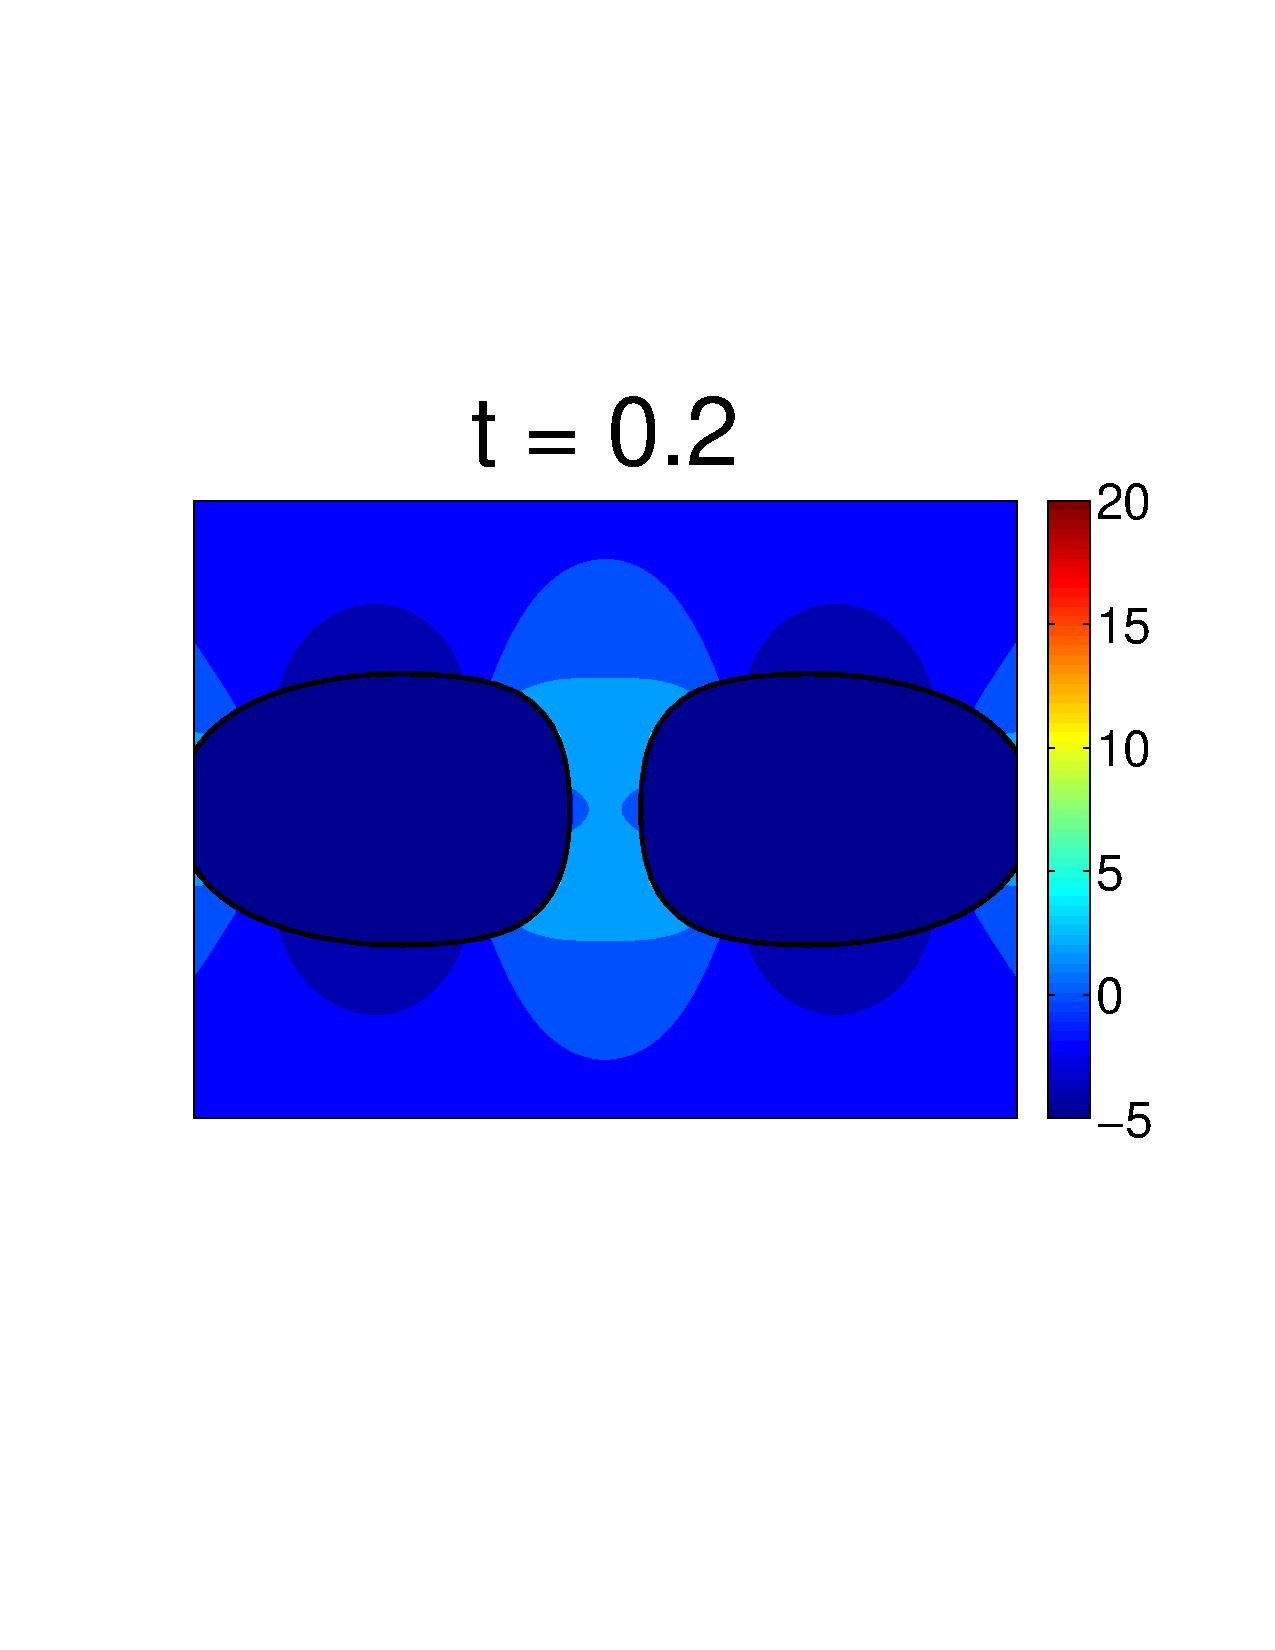
\includegraphics[trim=1.2cm 7cm 2cm 6cm,clip=true,scale = 0.15]{figs/pressureContourFrame01.pdf} &
  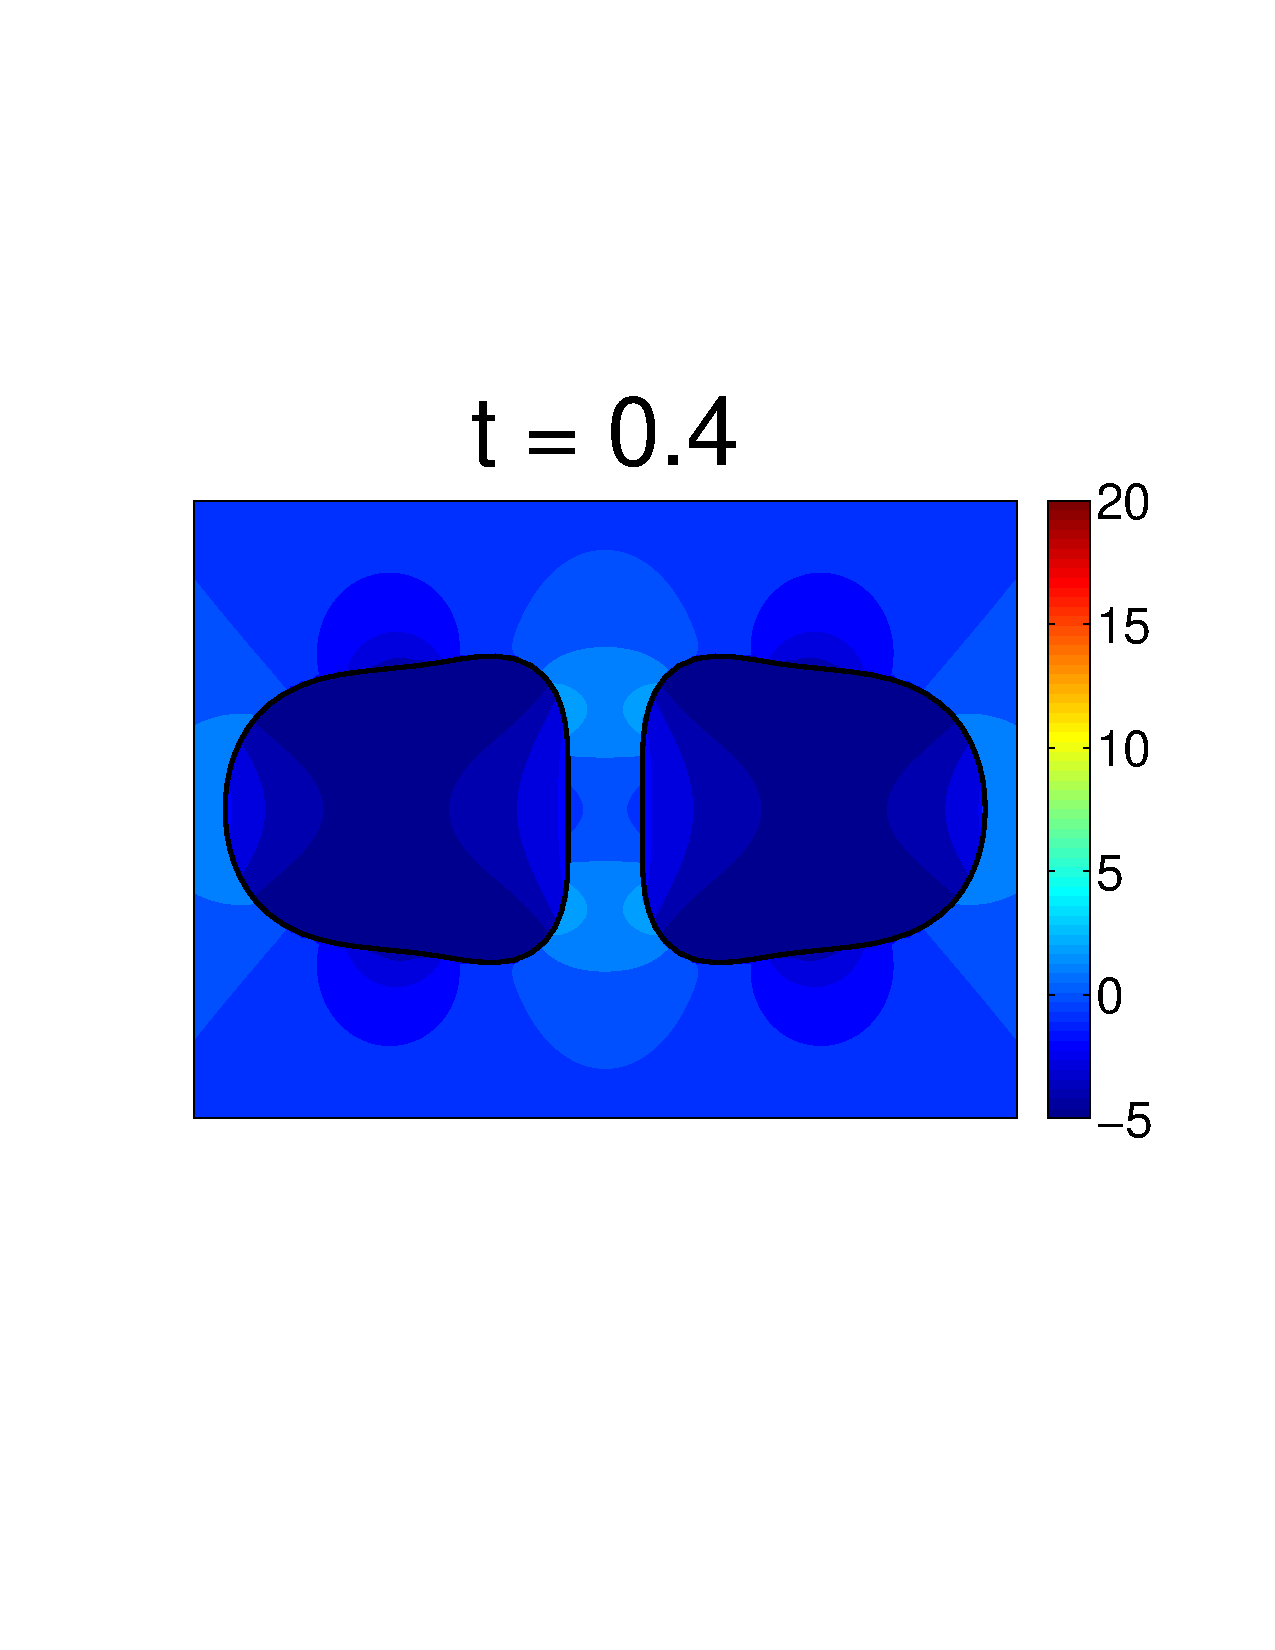
\includegraphics[trim=1.2cm 7cm 2cm 6cm,clip=true,scale = 0.15]{figs/pressureContourFrame02.pdf} &
  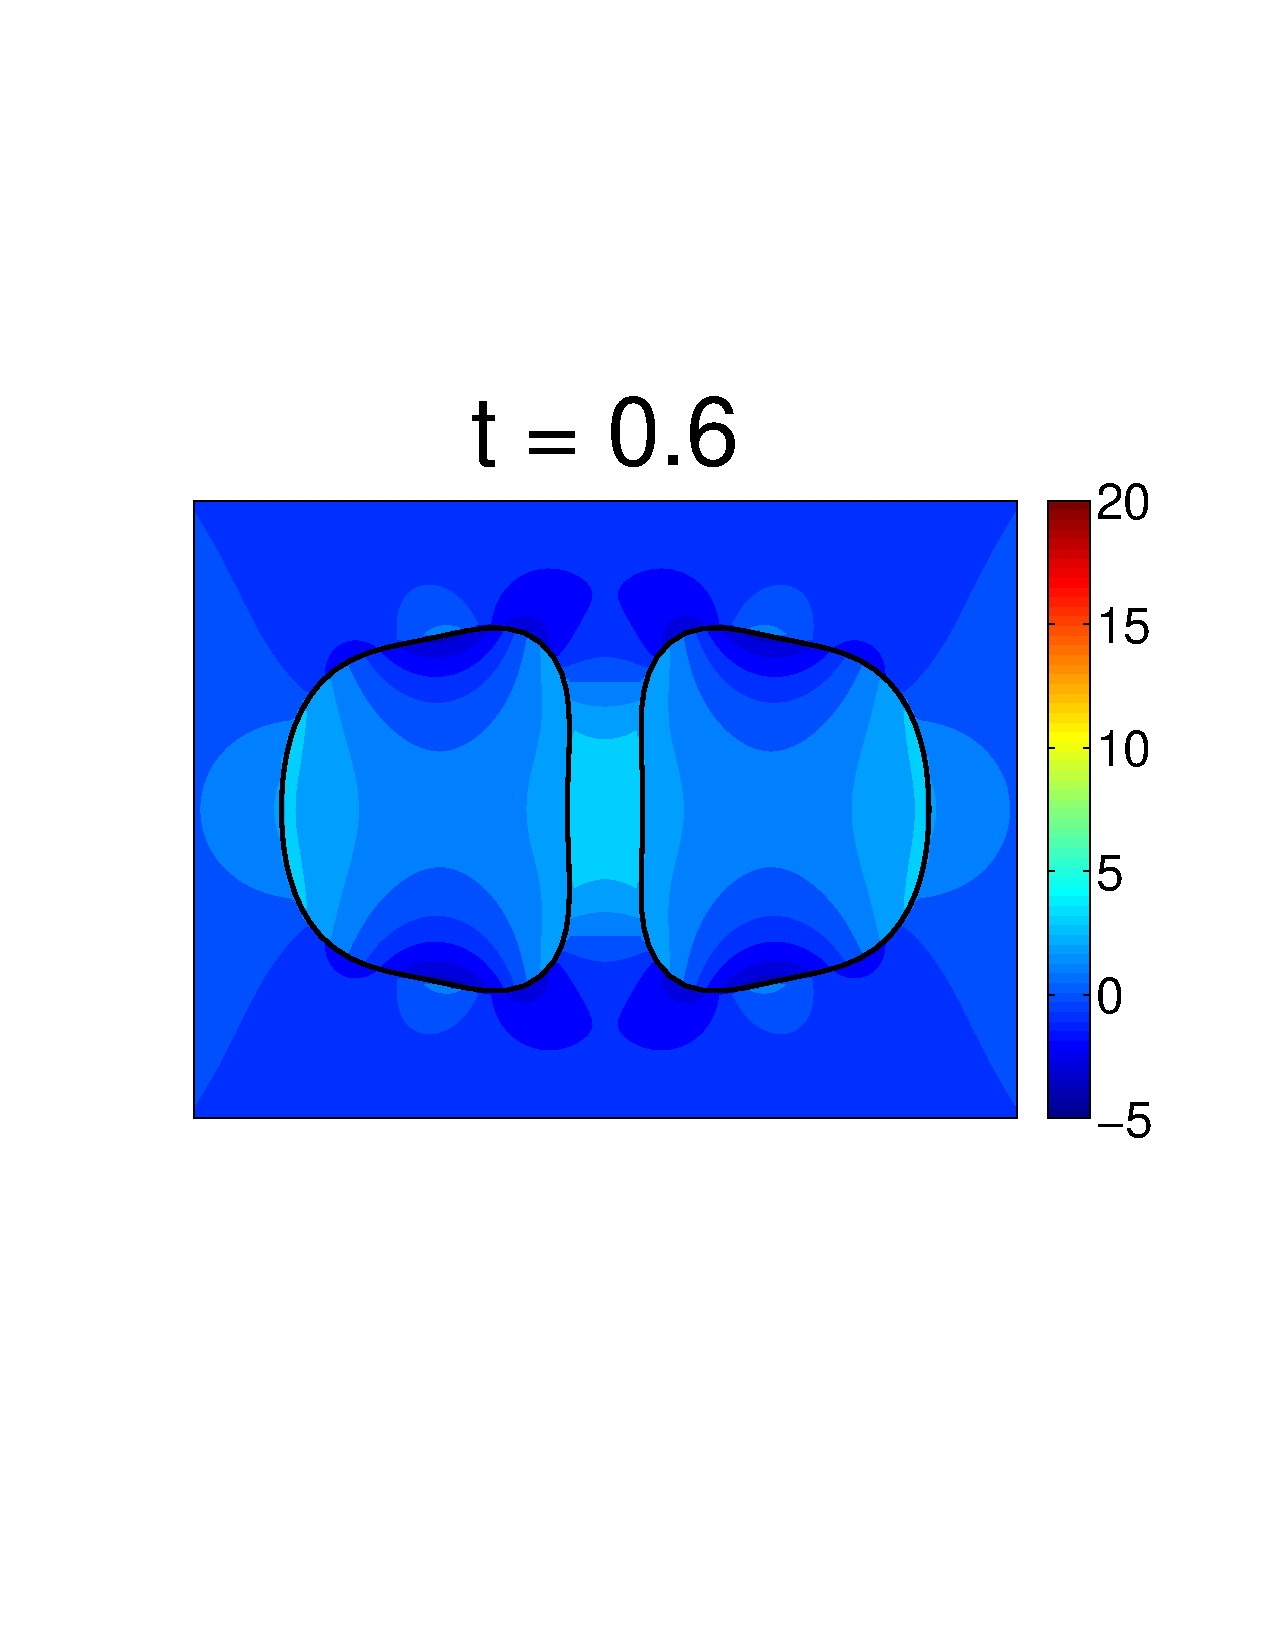
\includegraphics[trim=1.2cm 7cm 2cm 6cm,clip=true,scale = 0.15]{figs/pressureContourFrame03.pdf} &
  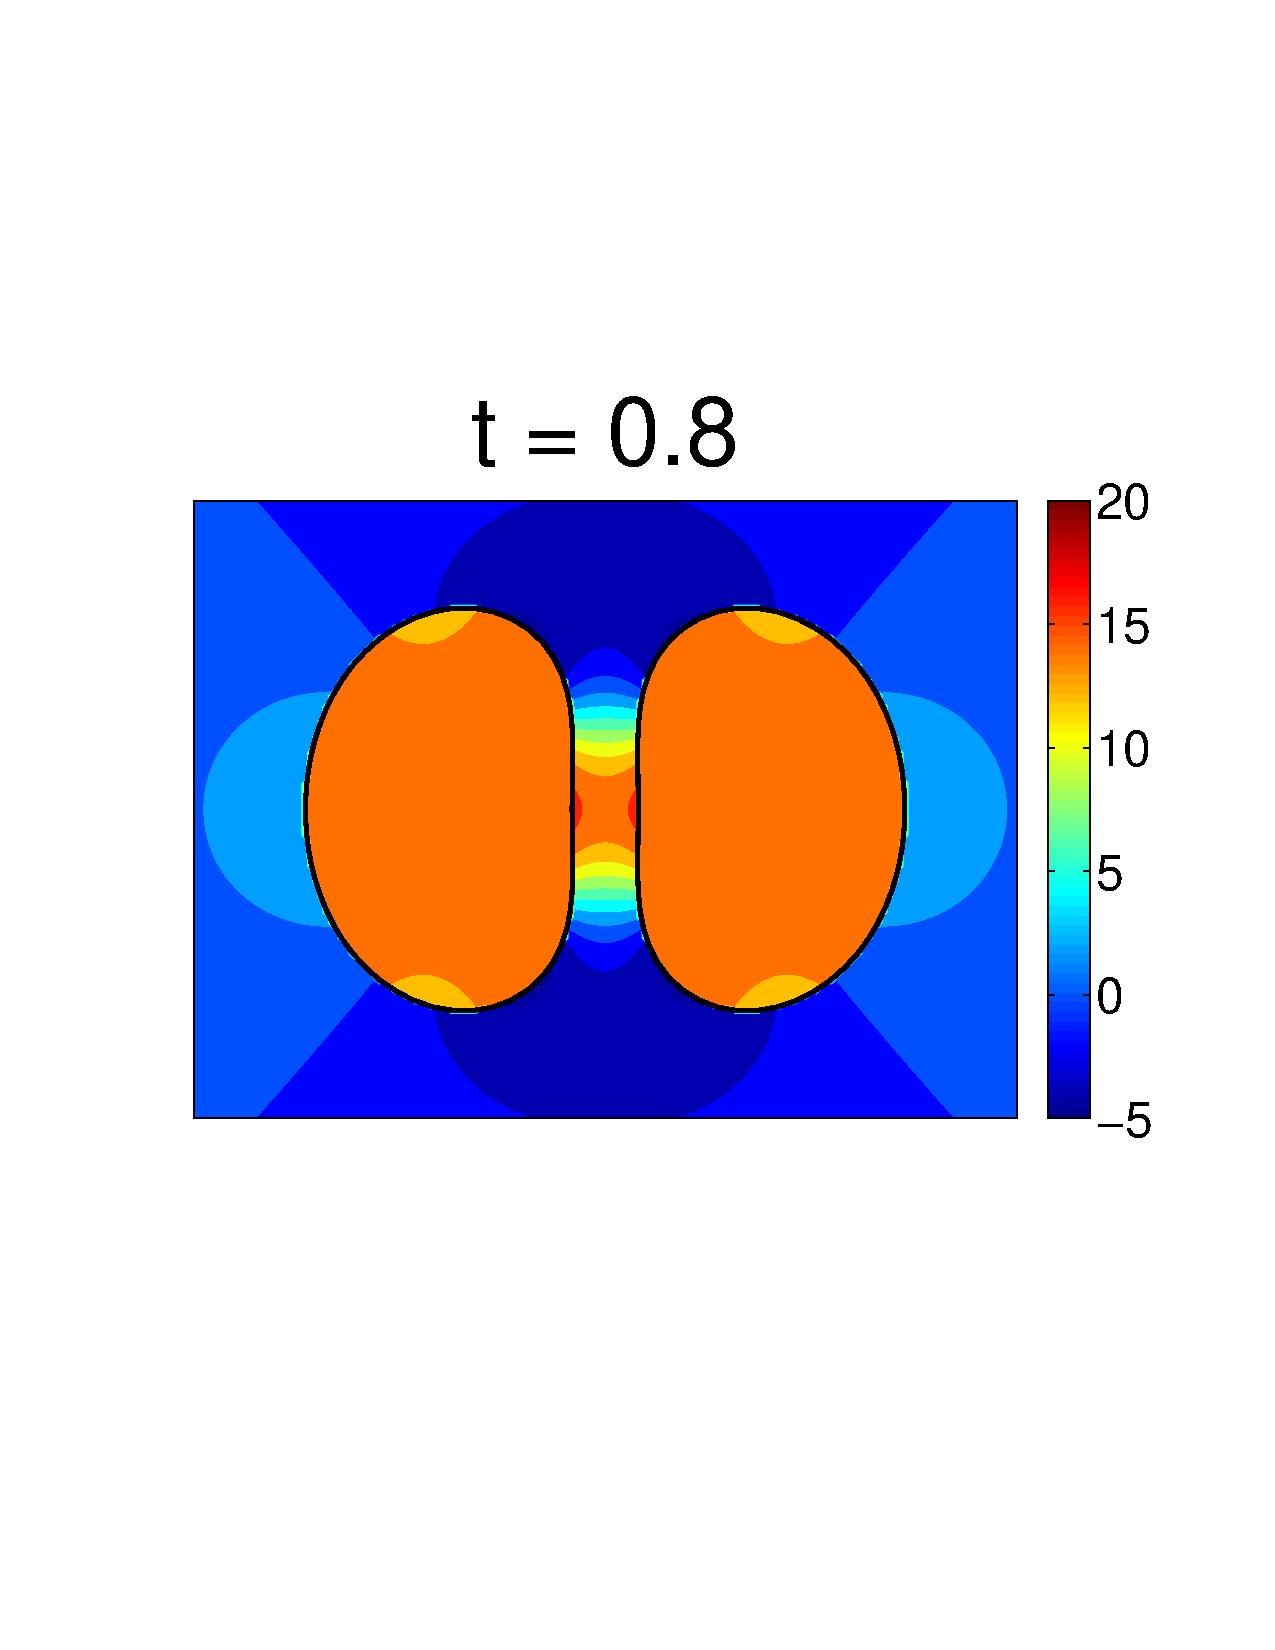
\includegraphics[trim=1.2cm 7cm 2cm 6cm,clip=true,scale = 0.15]{figs/pressureContourFrame04.pdf} &
  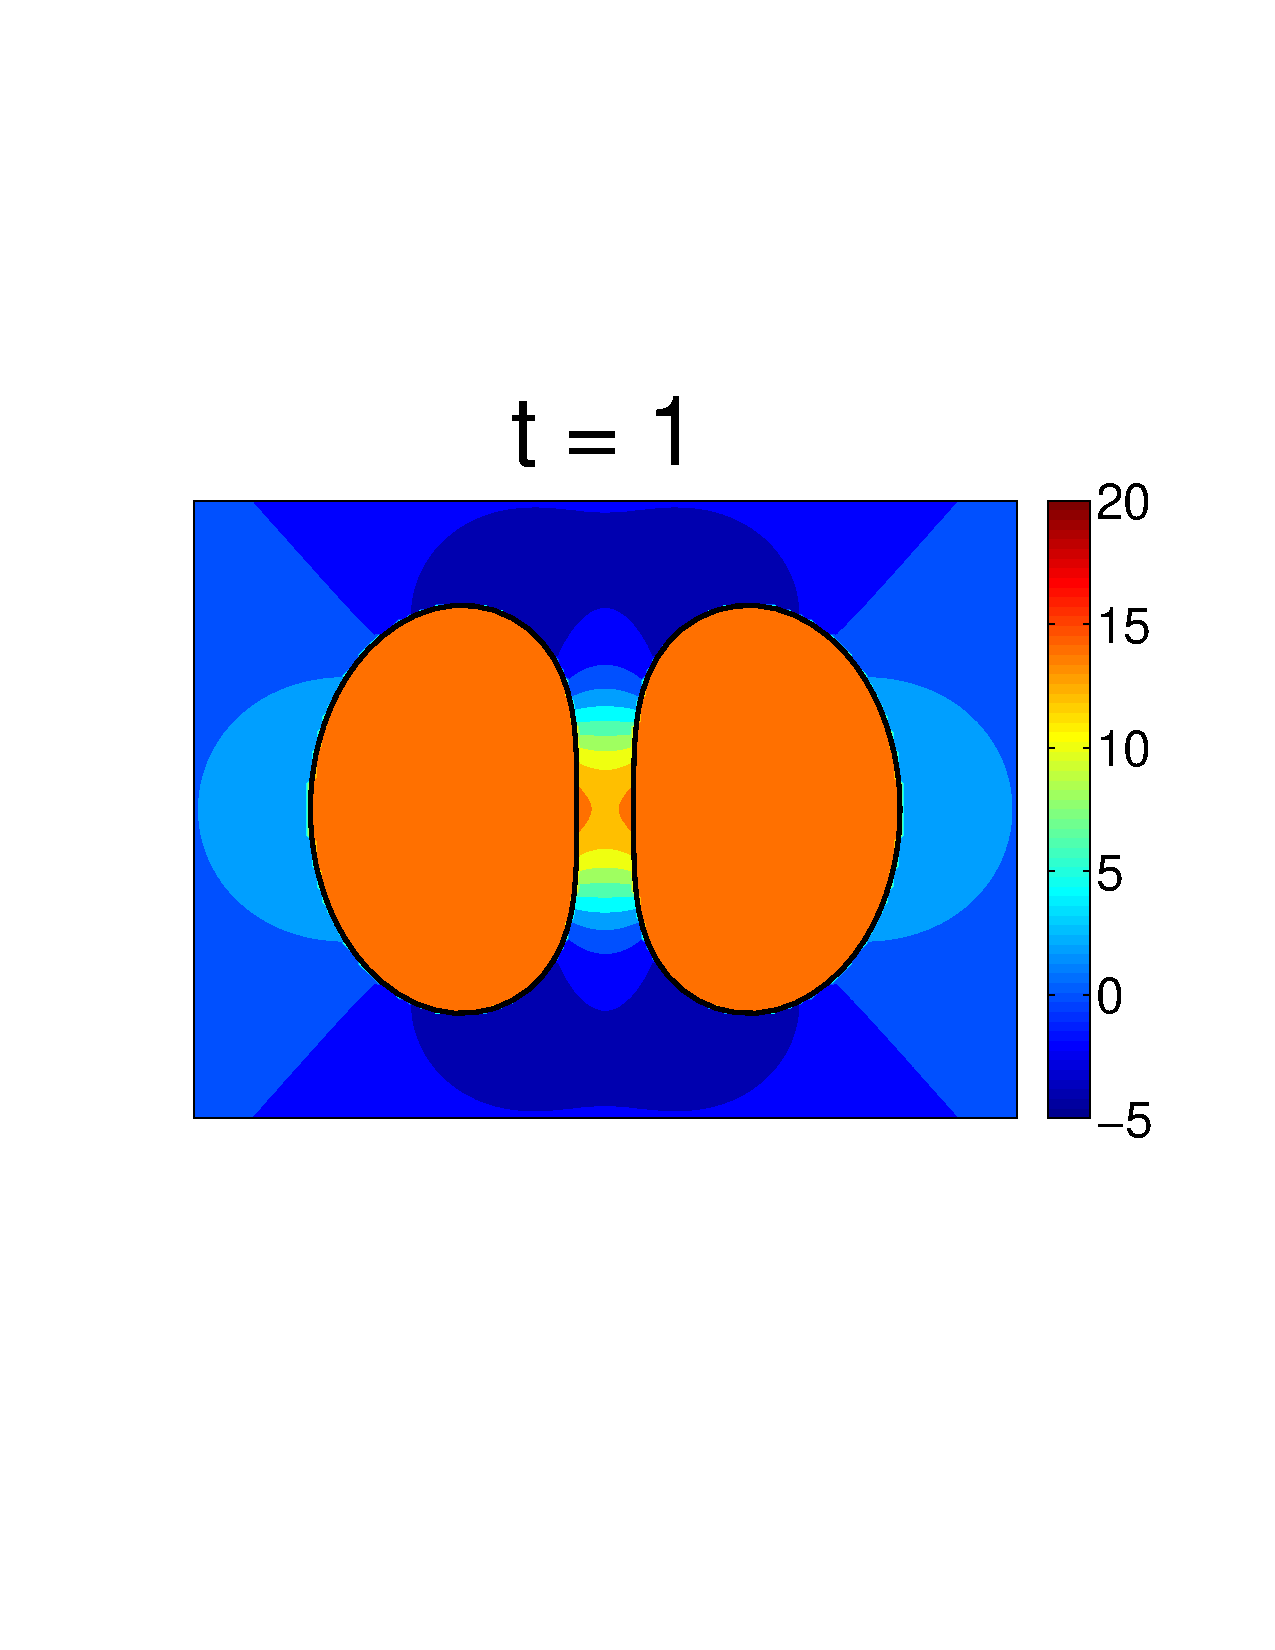
\includegraphics[trim=1.2cm 7cm 2cm 6cm,clip=true,scale = 0.15]{figs/pressureContourFrame05.pdf} \\ 
  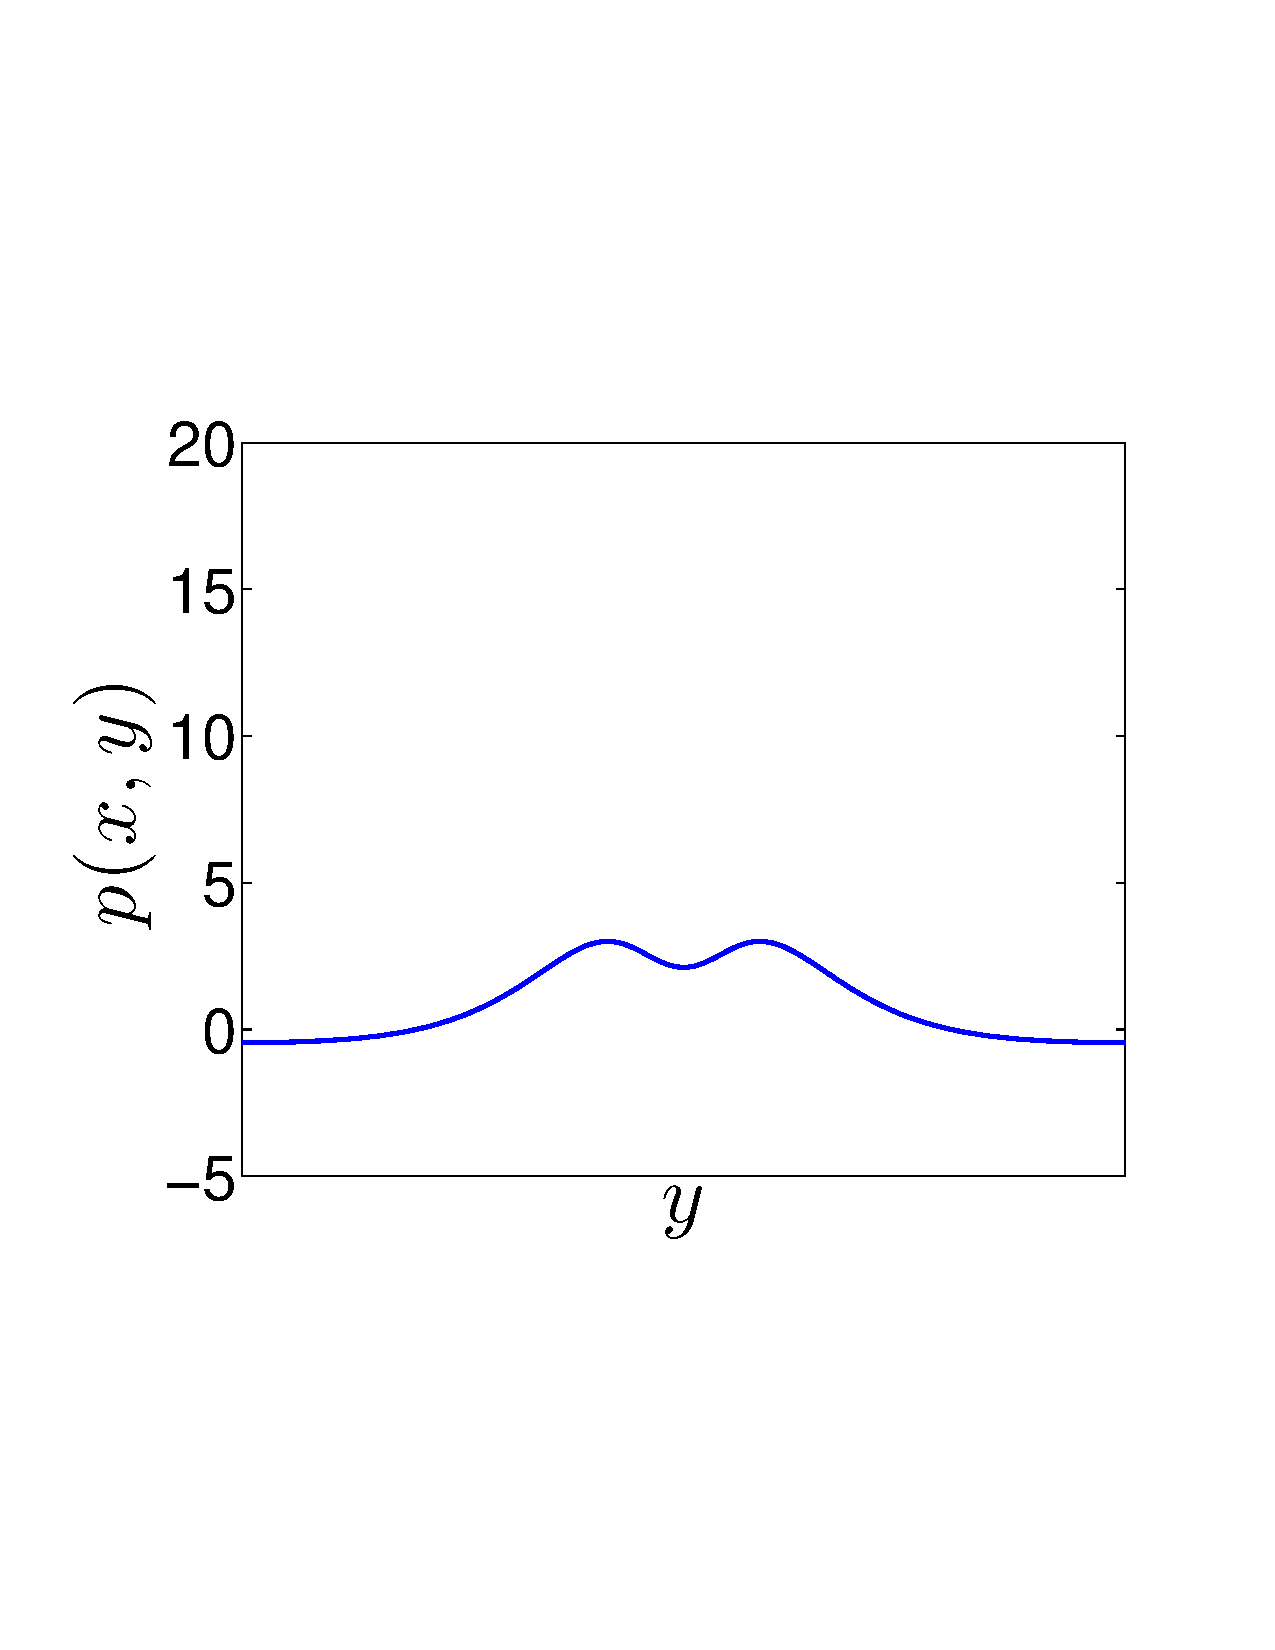
\includegraphics[trim=1.2cm 7cm 2cm 6cm,clip=true,scale = 0.15]{figs/pressurePlotFrame01.pdf} &
  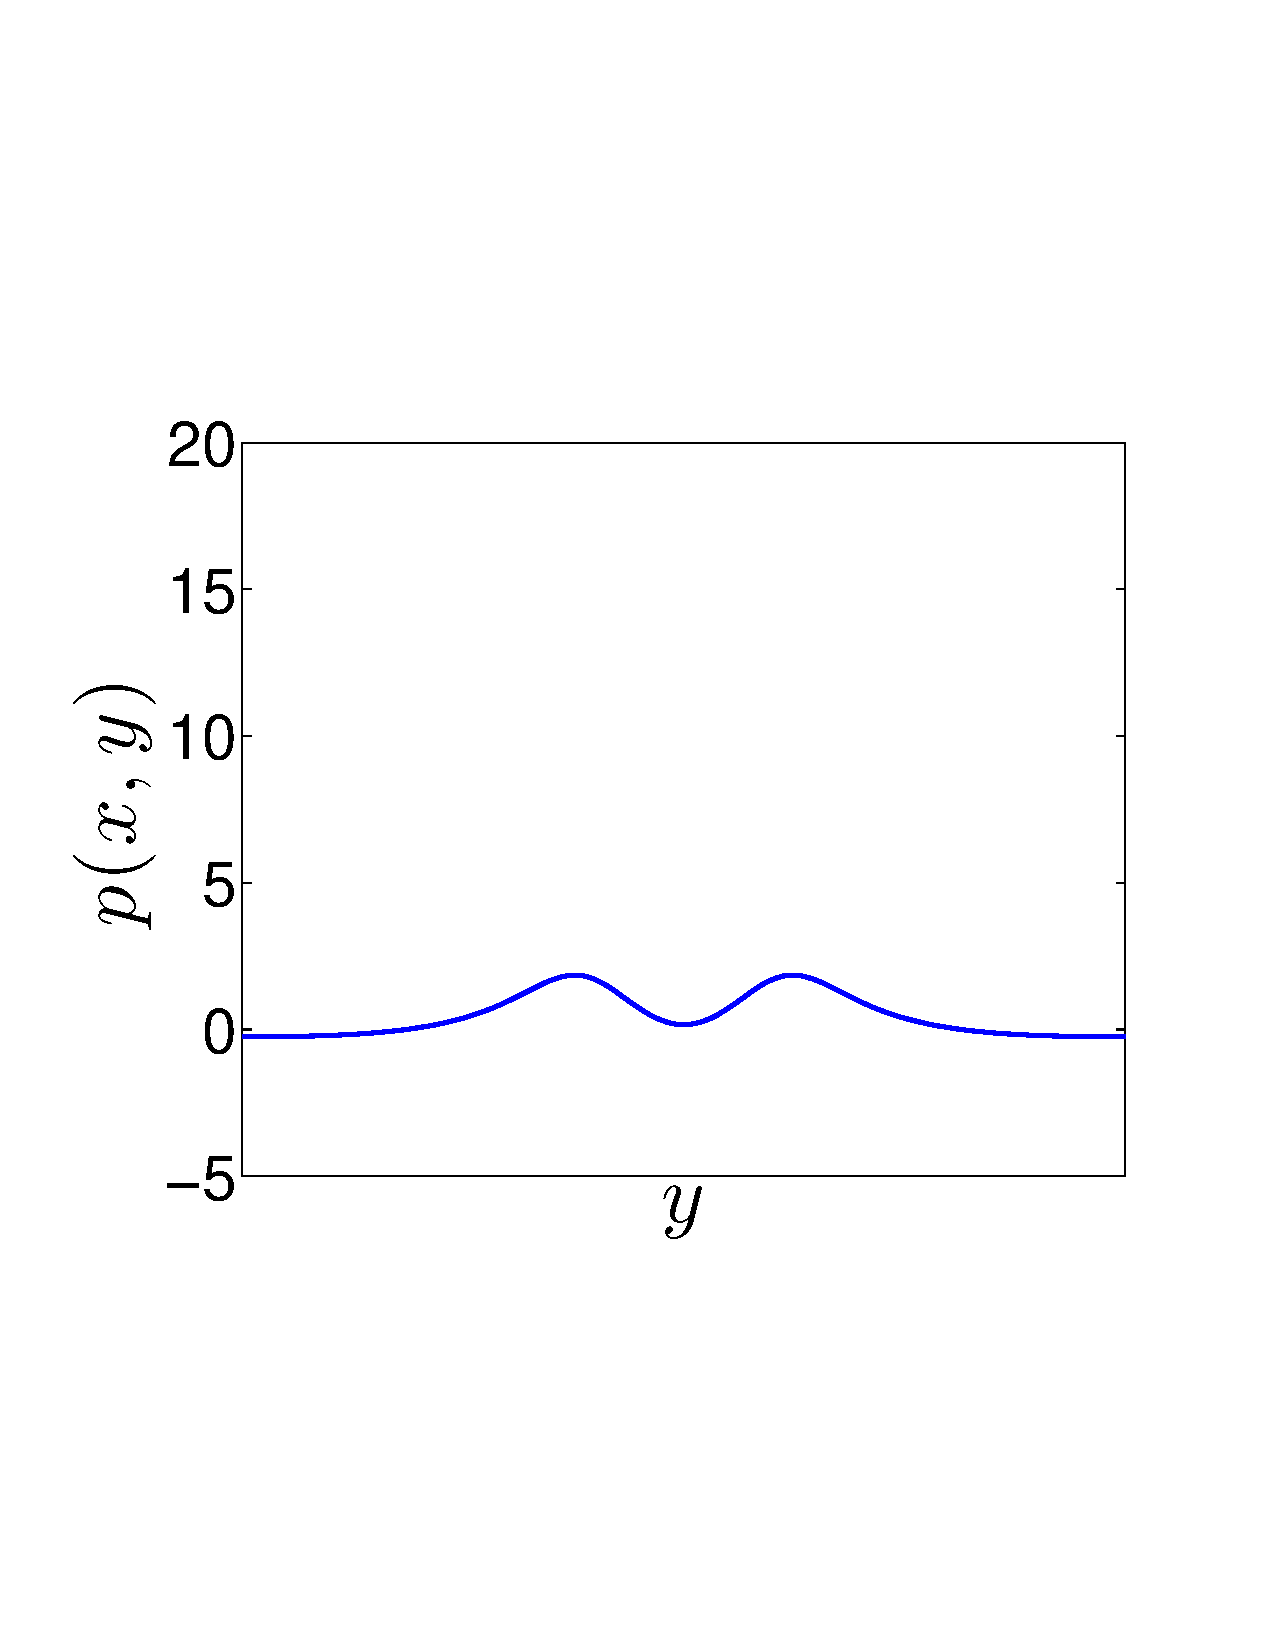
\includegraphics[trim=1.2cm 7cm 2cm 6cm,clip=true,scale = 0.15]{figs/pressurePlotFrame02.pdf} &
  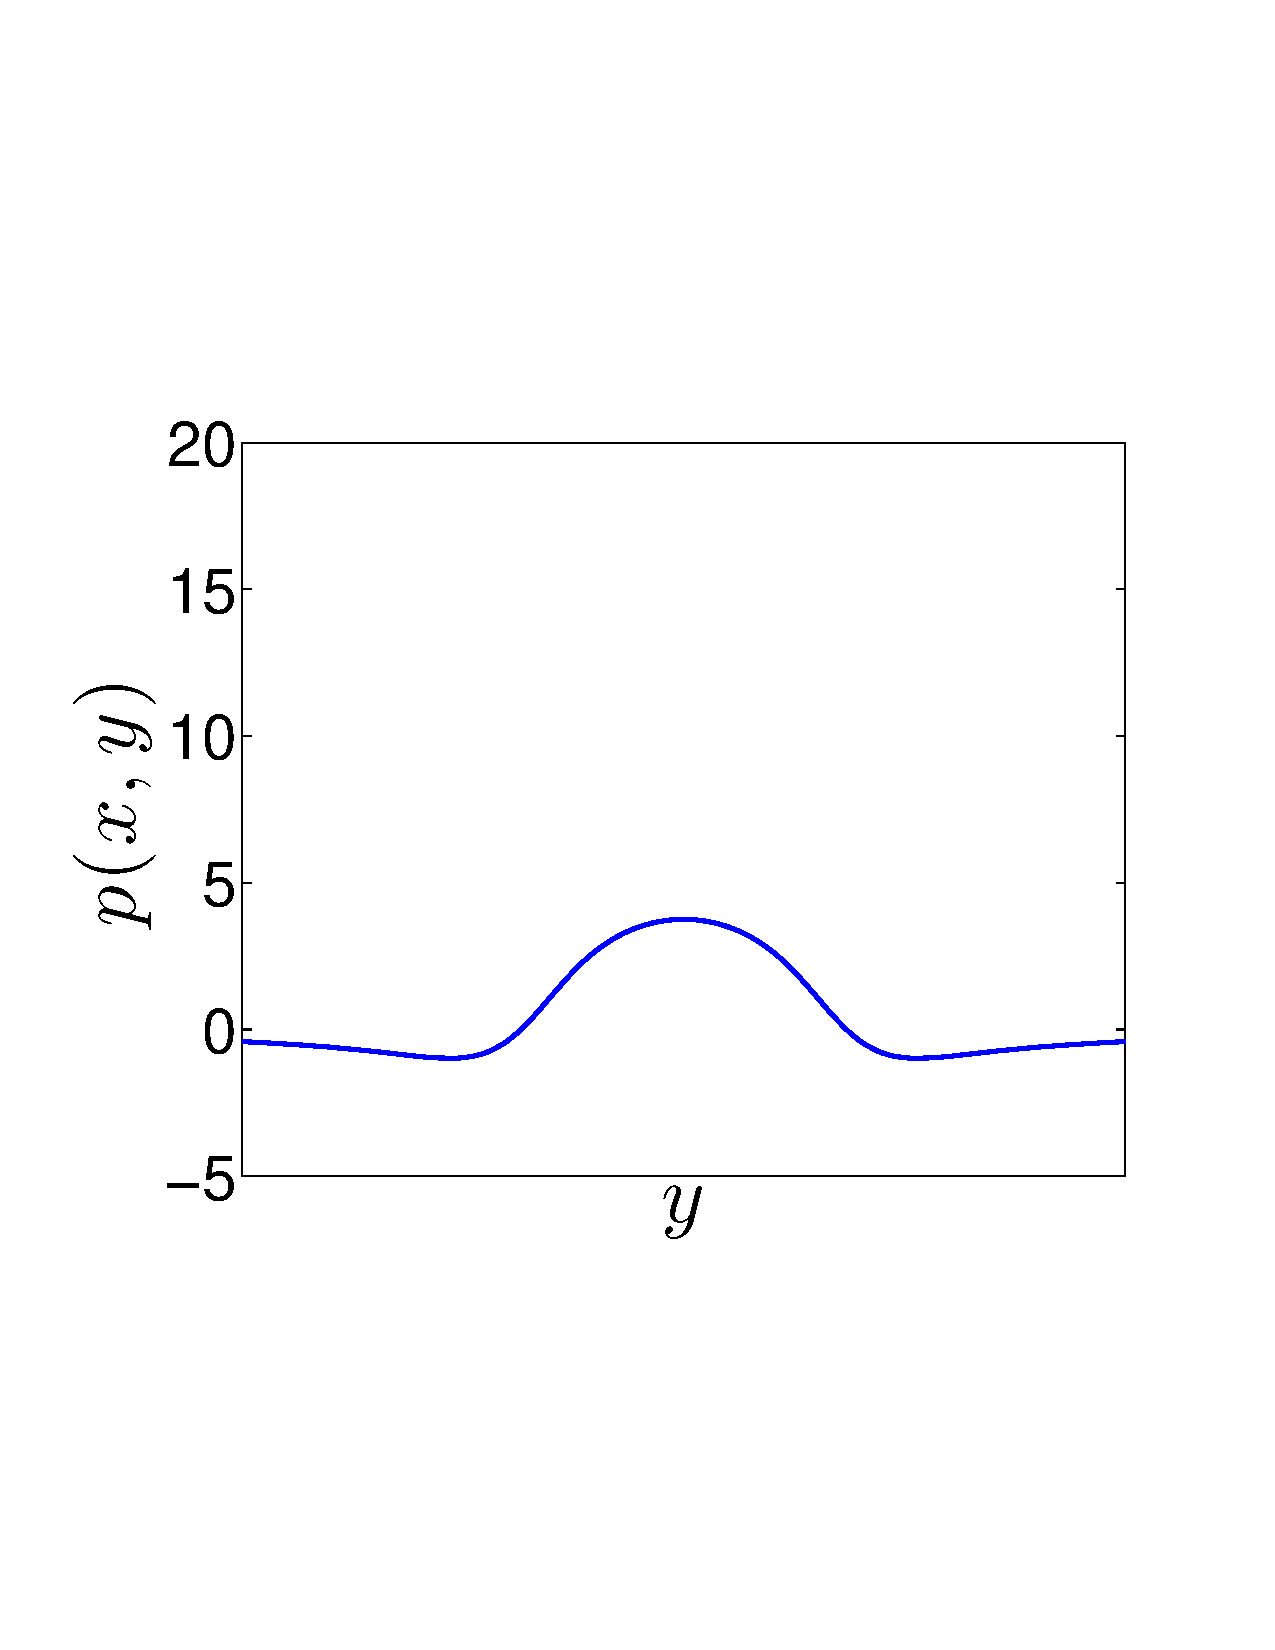
\includegraphics[trim=1.2cm 7cm 2cm 6cm,clip=true,scale = 0.15]{figs/pressurePlotFrame03.pdf} &
  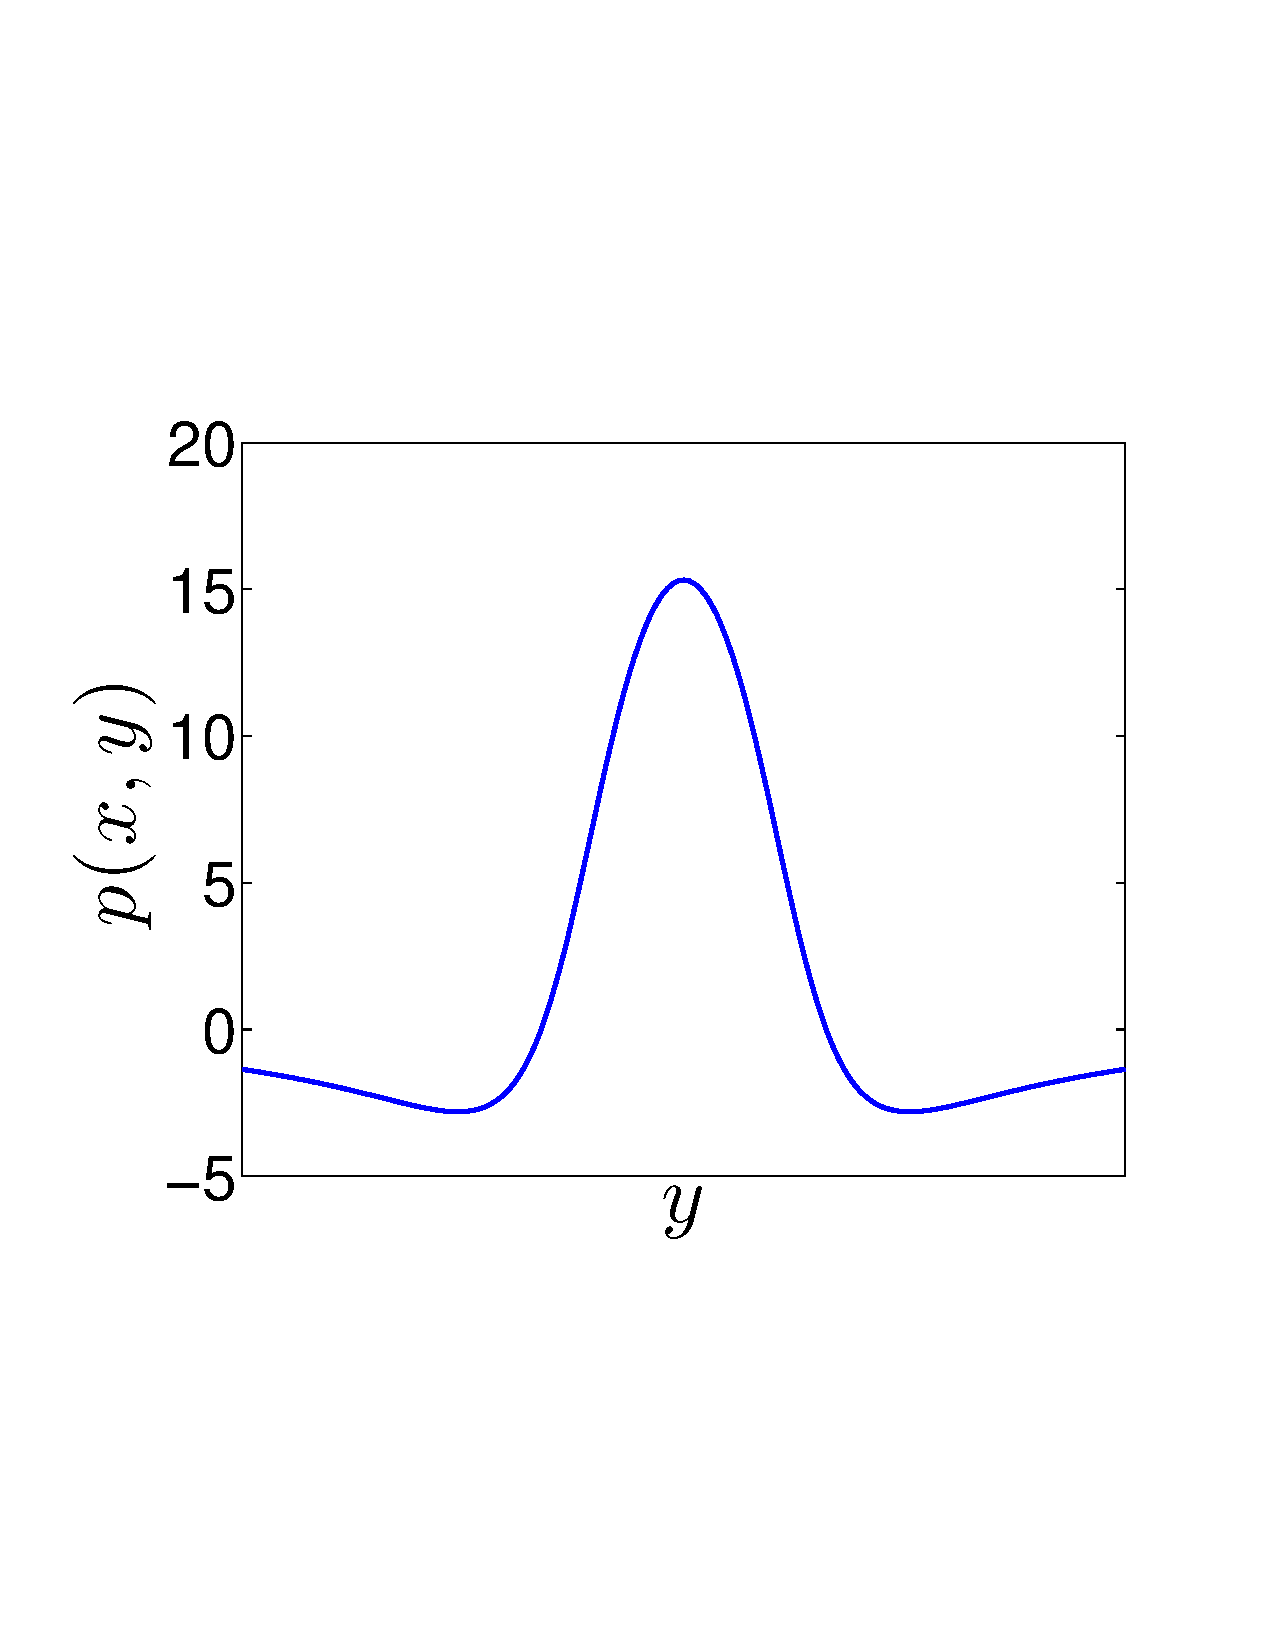
\includegraphics[trim=1.2cm 7cm 2cm 6cm,clip=true,scale = 0.15]{figs/pressurePlotFrame04.pdf} &
  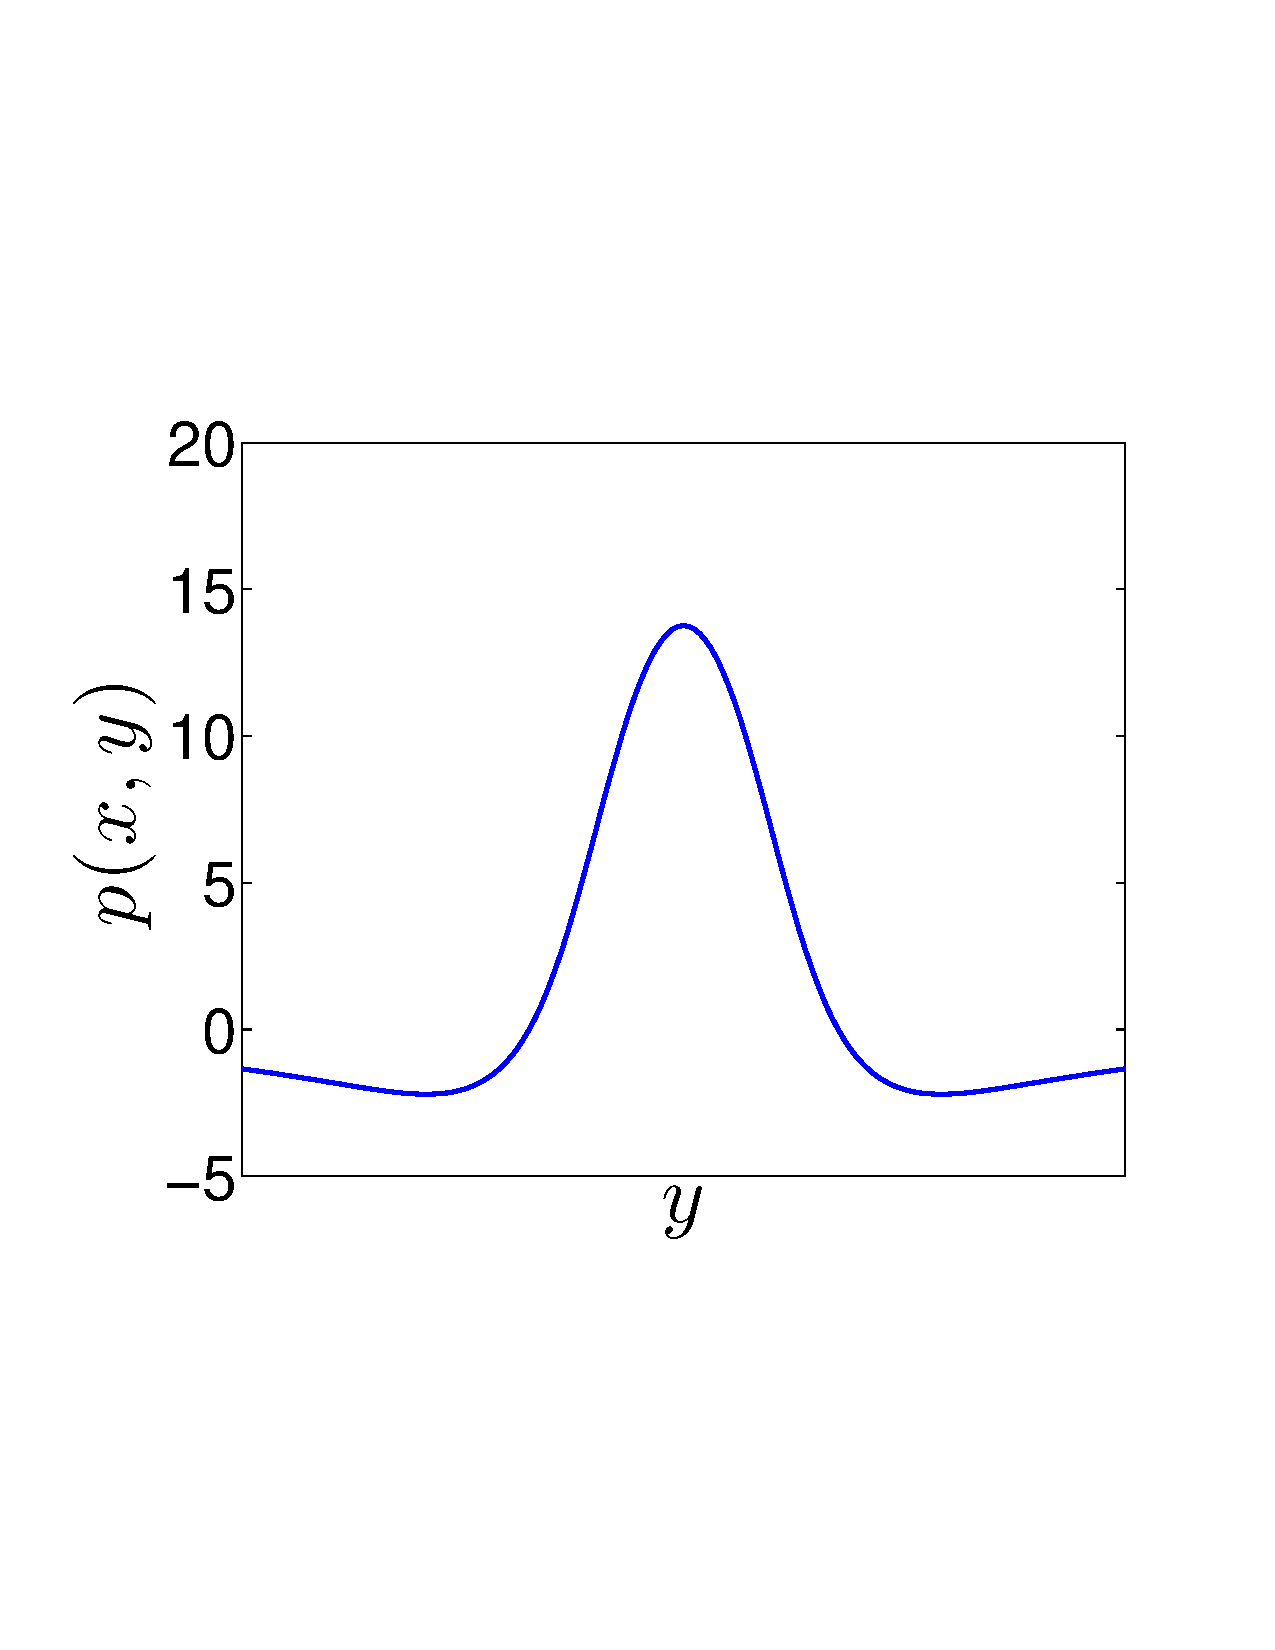
\includegraphics[trim=1.2cm 7cm 2cm 6cm,clip=true,scale = 0.15]{figs/pressurePlotFrame05.pdf} \\ \\ 
  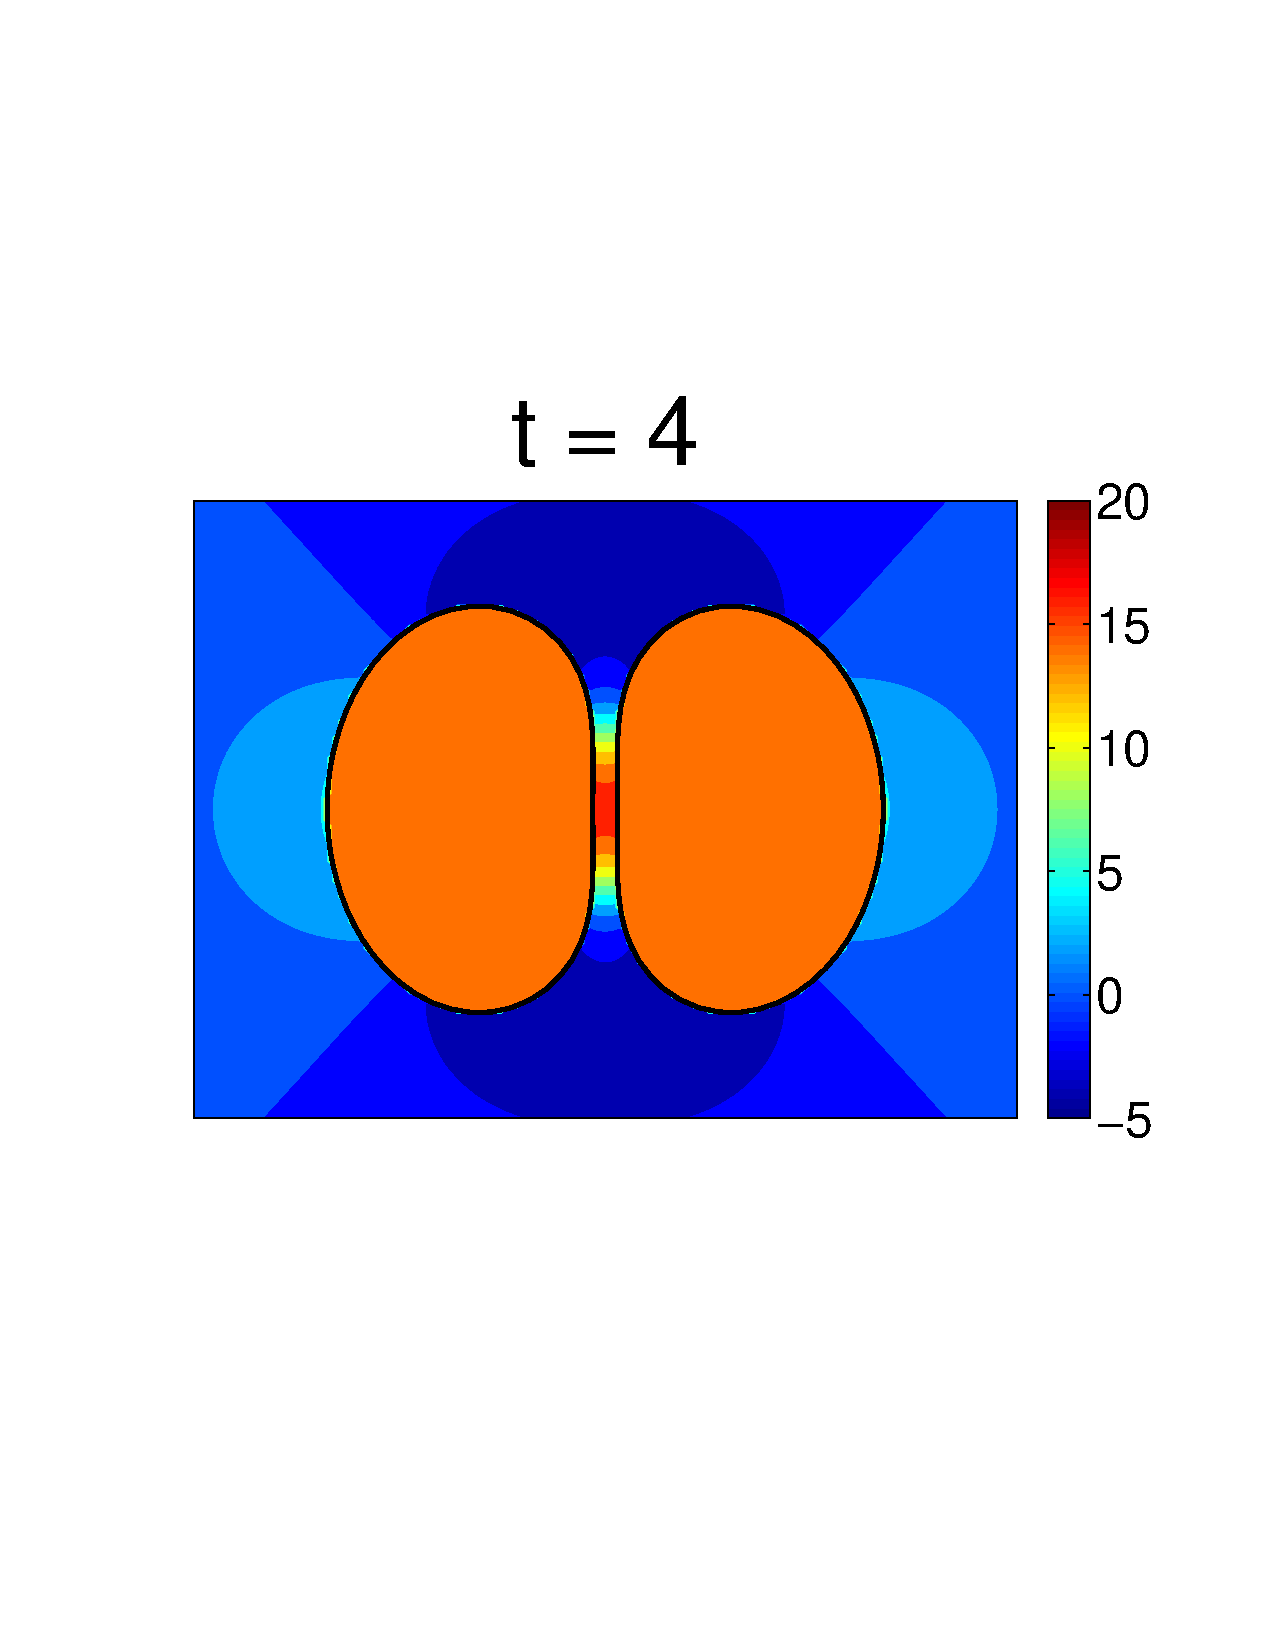
\includegraphics[trim=1.2cm 7cm 2cm 6cm,clip=true,scale = 0.15]{figs/pressureContourFrame06.pdf} &
  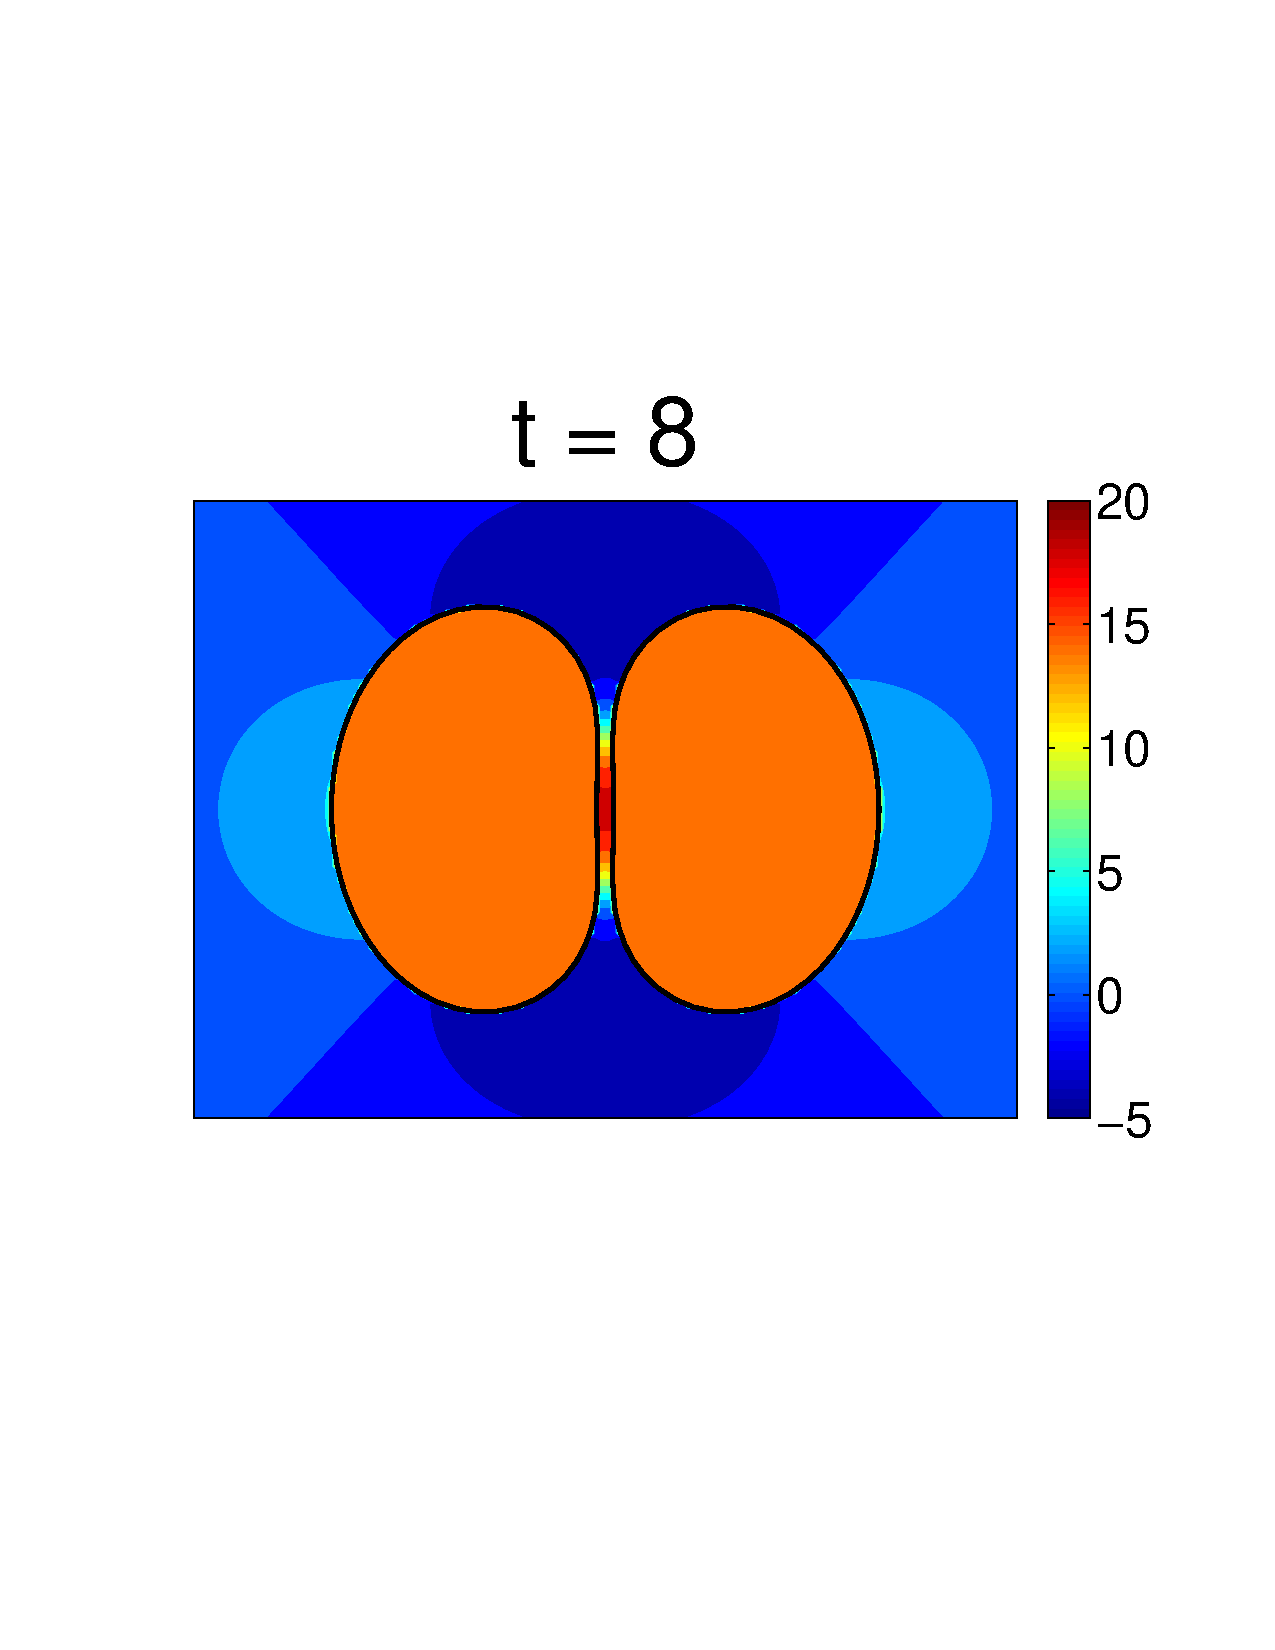
\includegraphics[trim=1.2cm 7cm 2cm 6cm,clip=true,scale = 0.15]{figs/pressureContourFrame07.pdf} &
  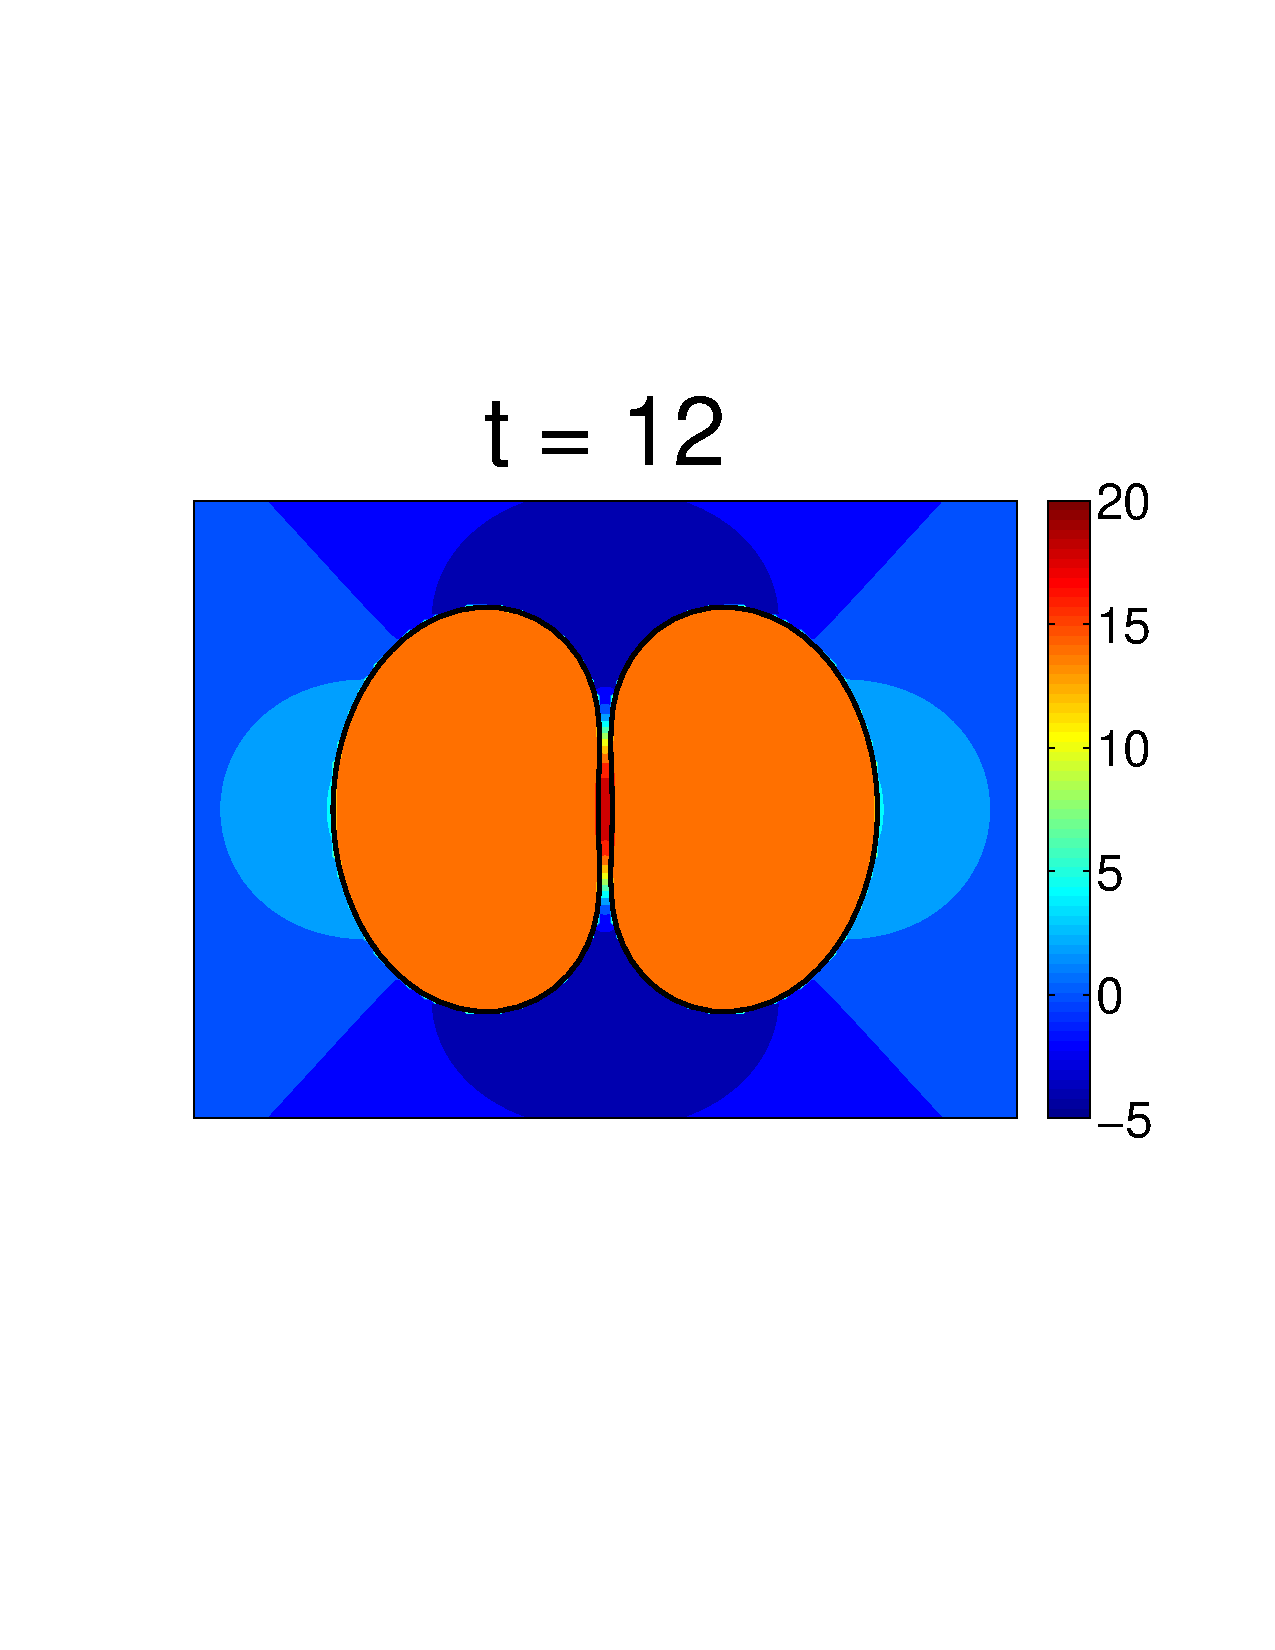
\includegraphics[trim=1.2cm 7cm 2cm 6cm,clip=true,scale = 0.15]{figs/pressureContourFrame08.pdf} &
  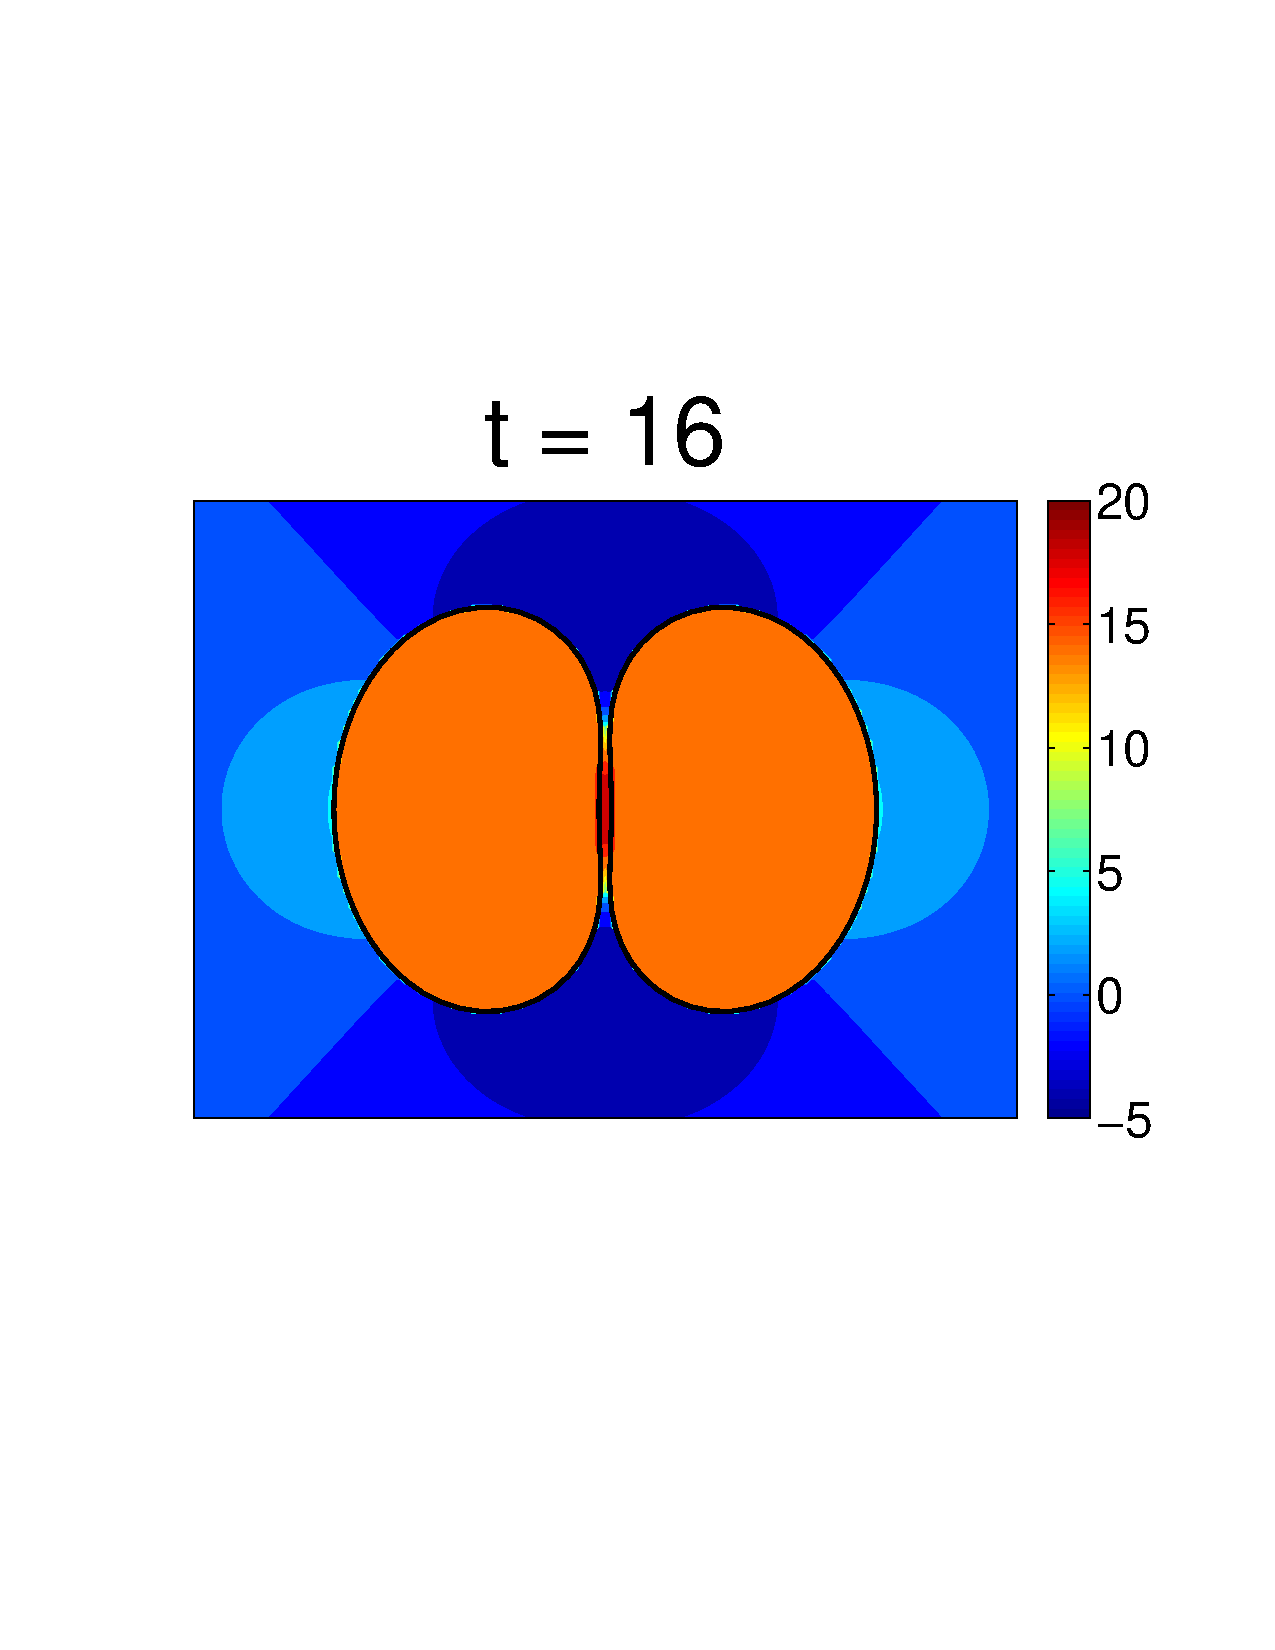
\includegraphics[trim=1.2cm 7cm 2cm 6cm,clip=true,scale = 0.15]{figs/pressureContourFrame09.pdf} &
  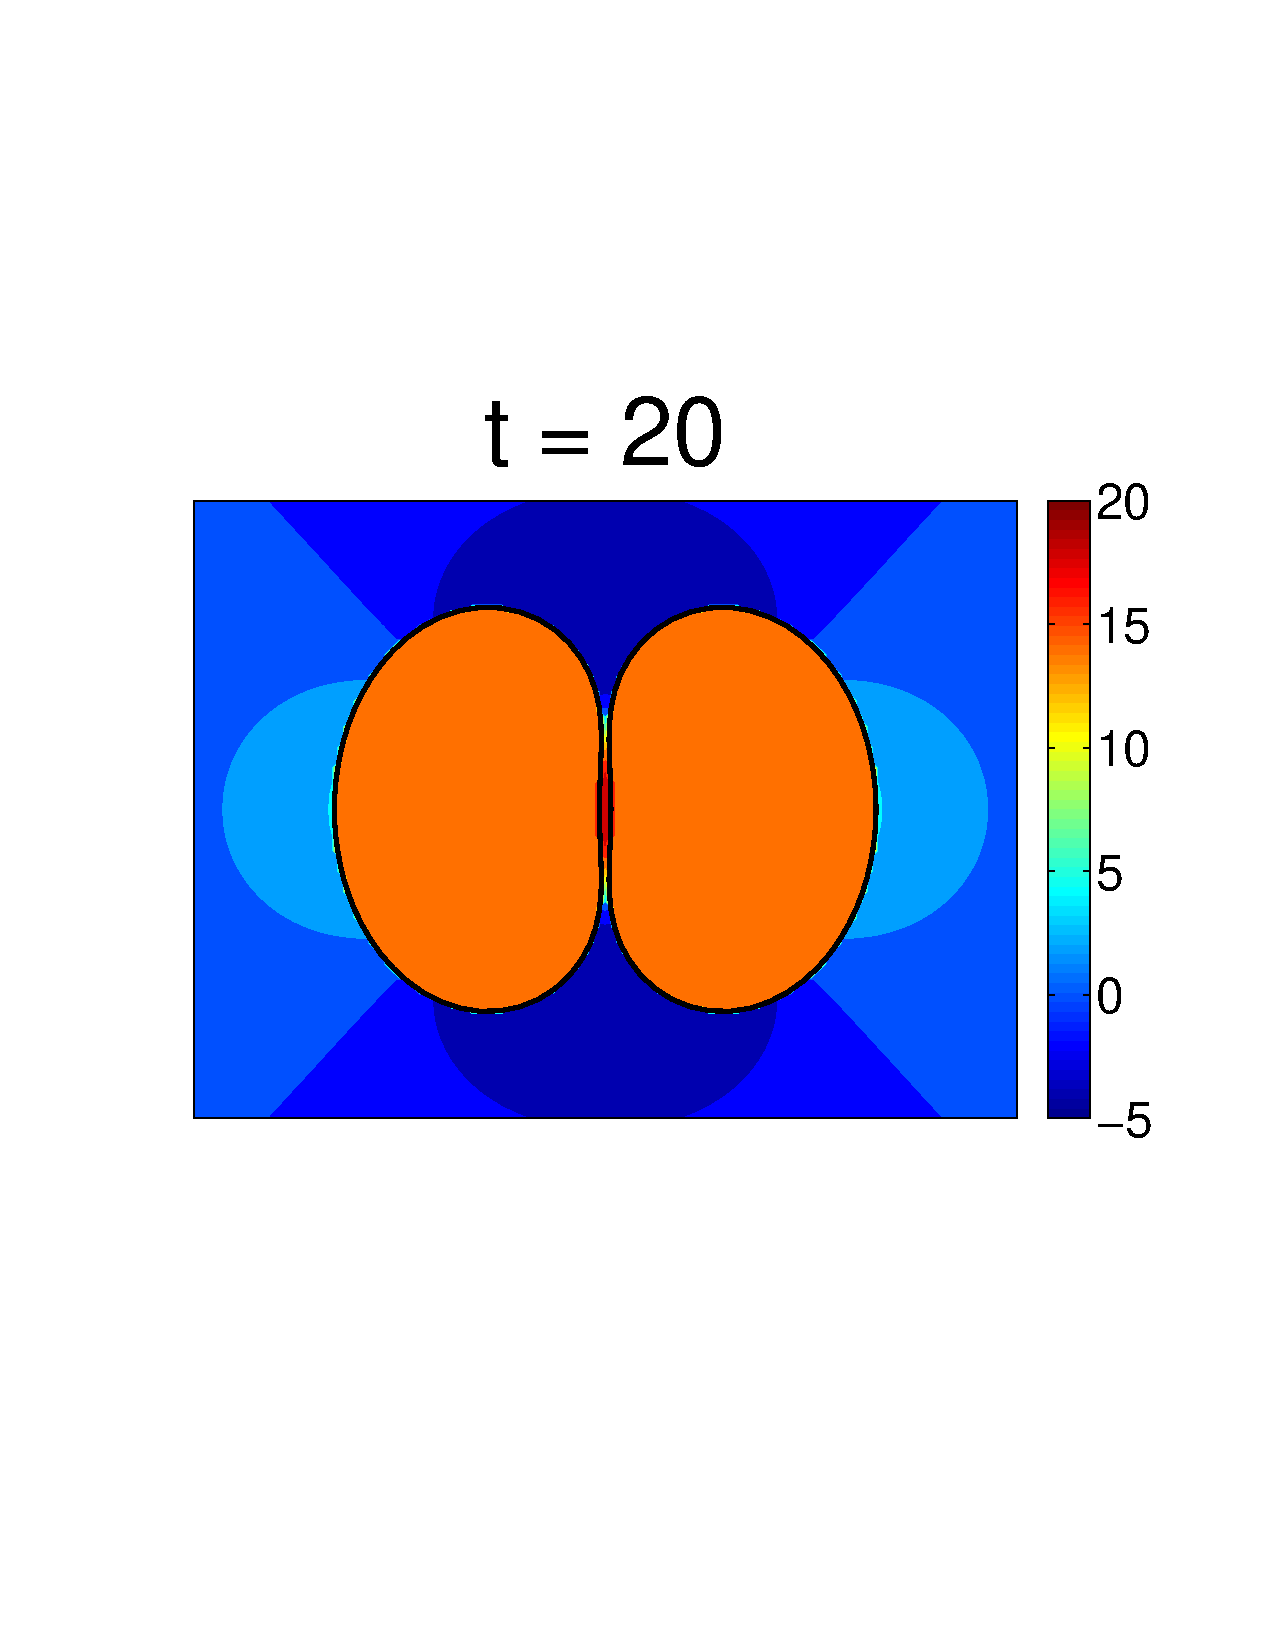
\includegraphics[trim=1.2cm 7cm 2cm 6cm,clip=true,scale = 0.15]{figs/pressureContourFrame10.pdf} \\ 
  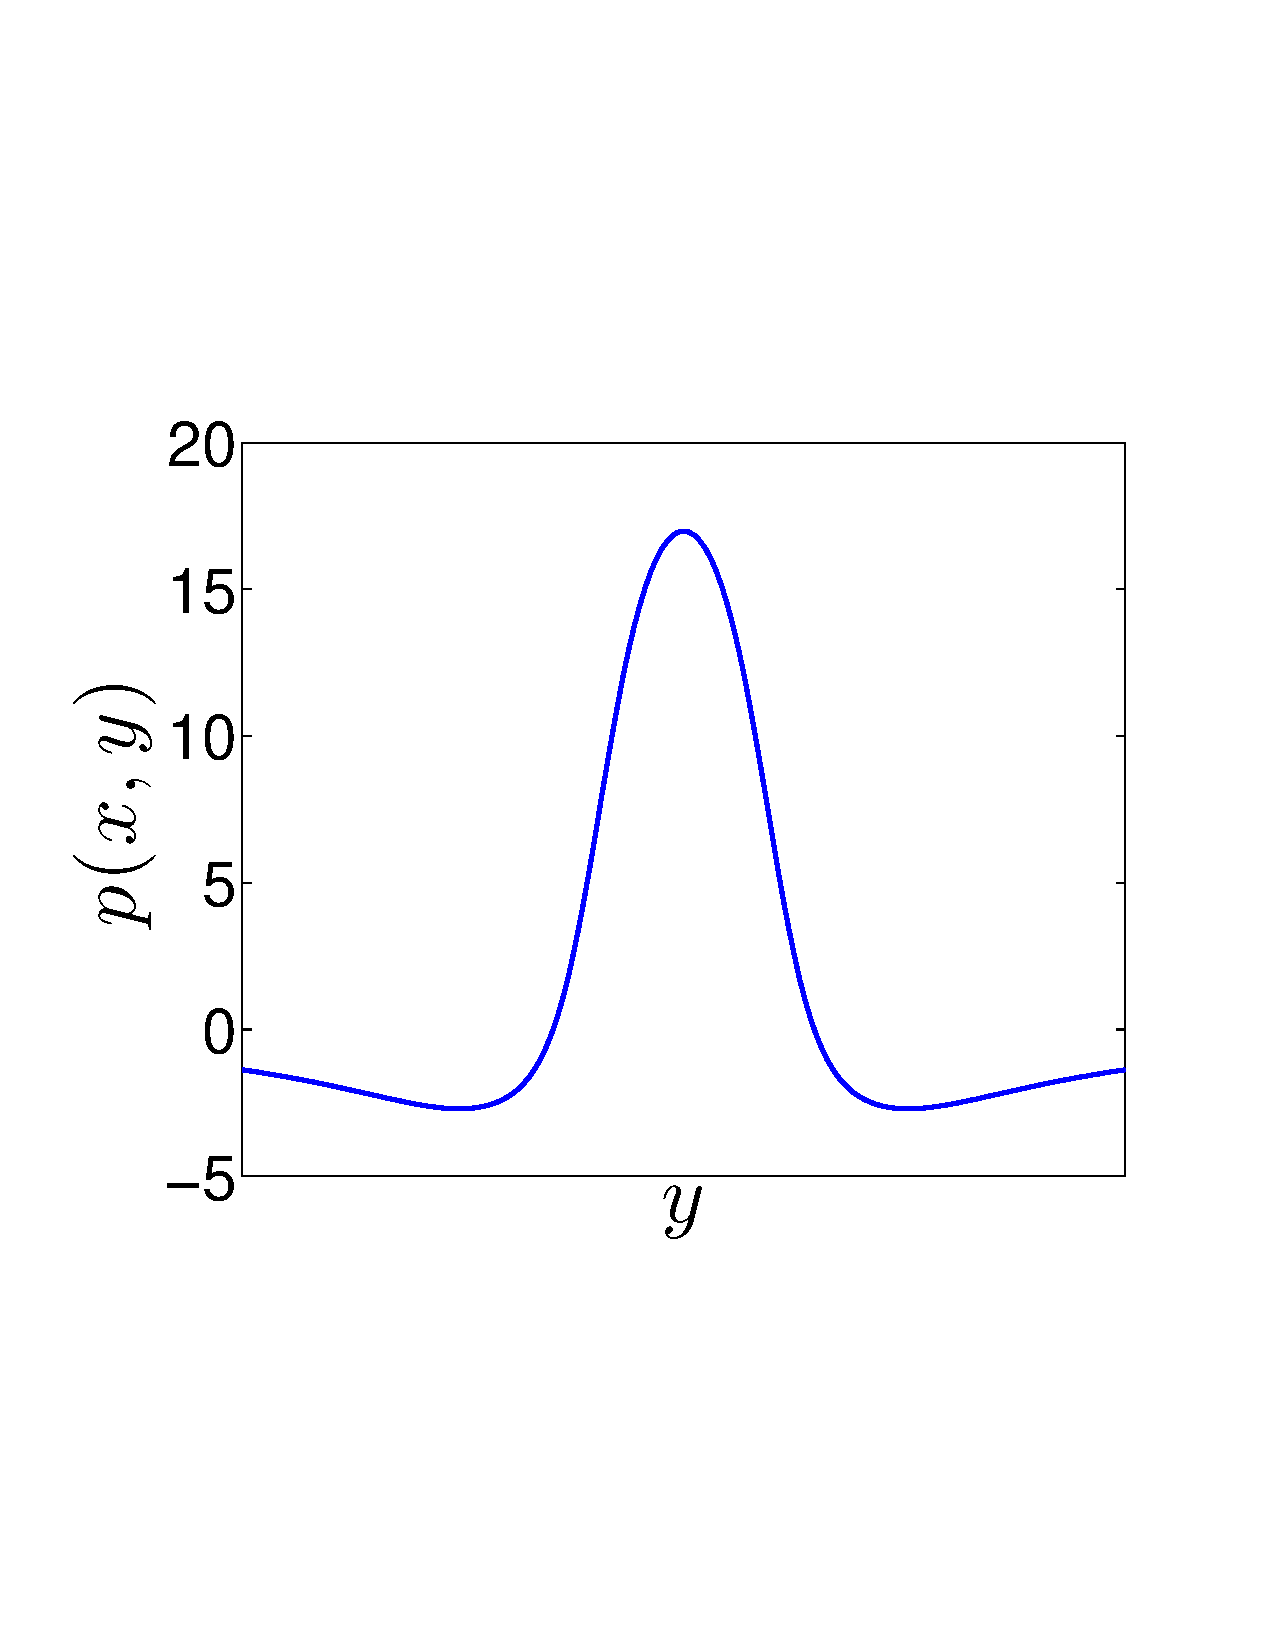
\includegraphics[trim=1.2cm 7cm 2cm 6cm,clip=true,scale = 0.15]{figs/pressurePlotFrame06.pdf} &
  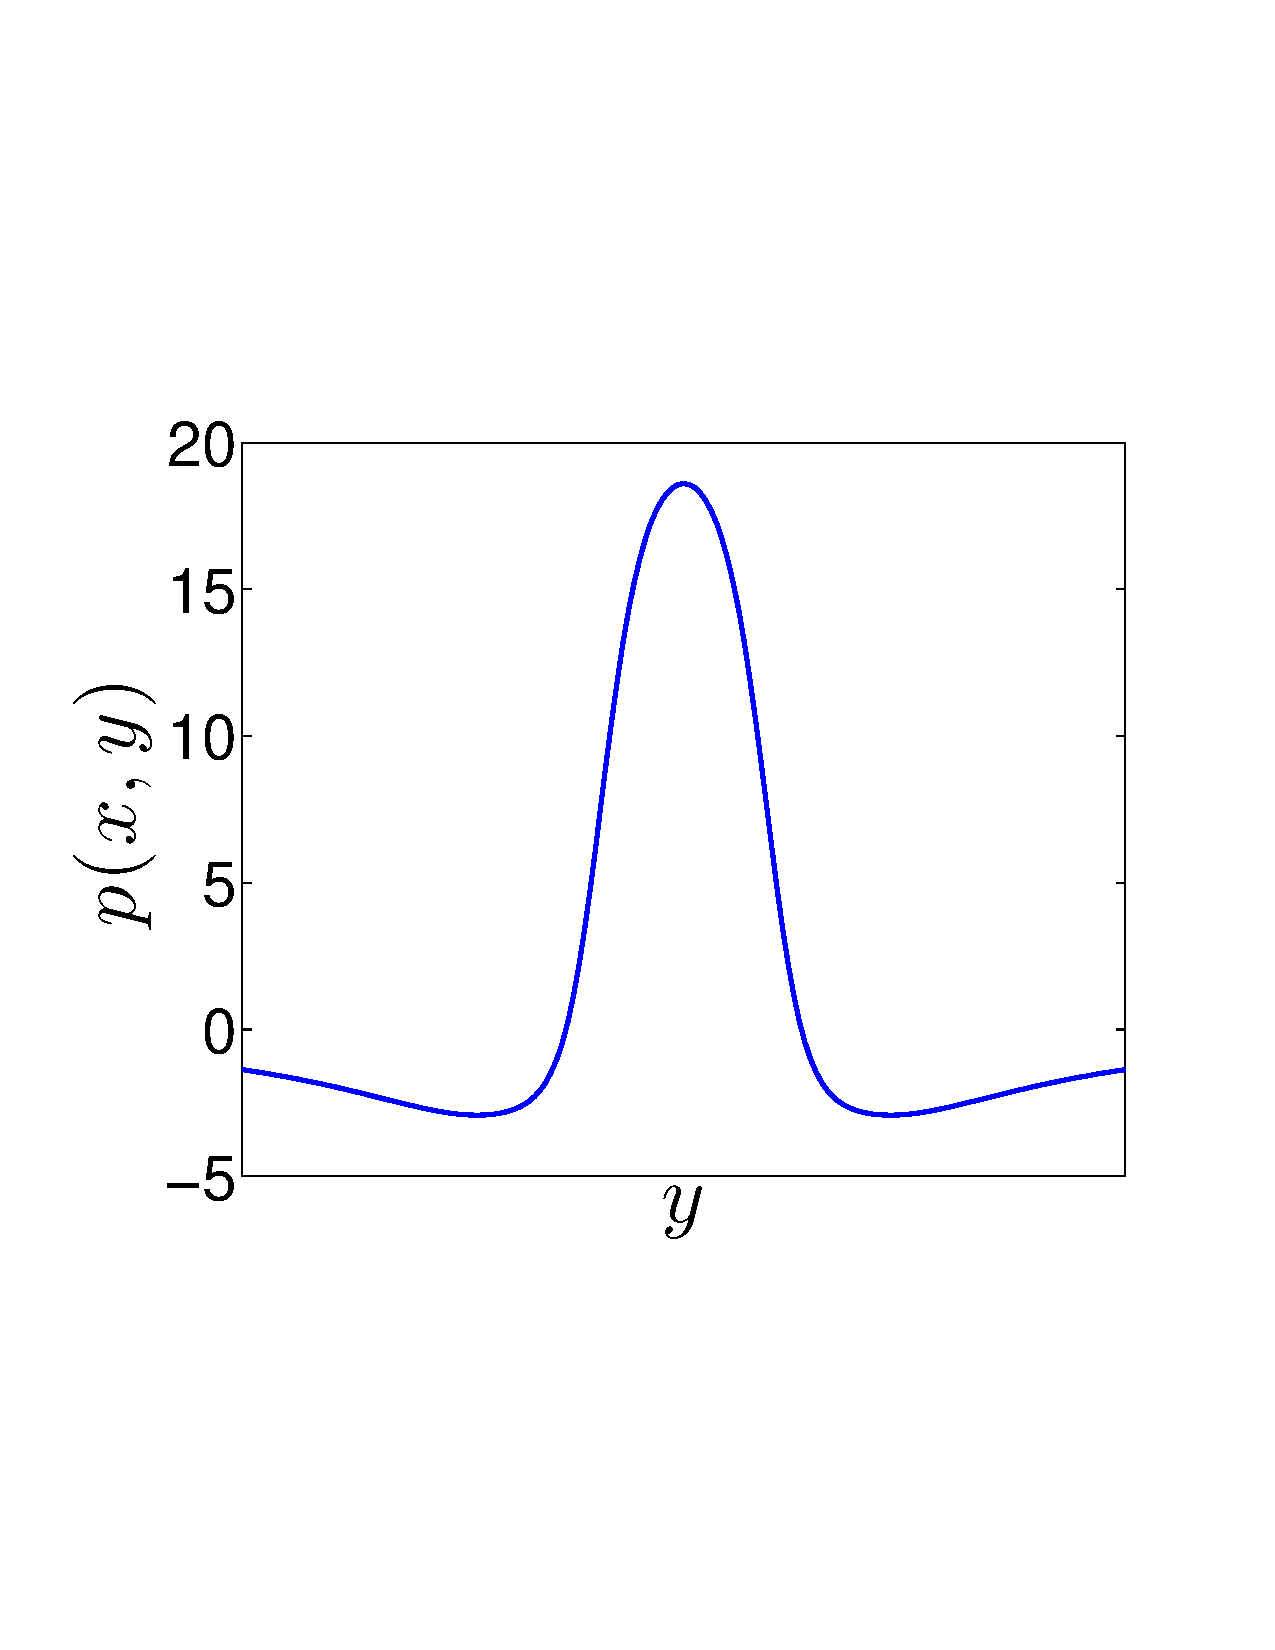
\includegraphics[trim=1.2cm 7cm 2cm 6cm,clip=true,scale = 0.15]{figs/pressurePlotFrame07.pdf} &
  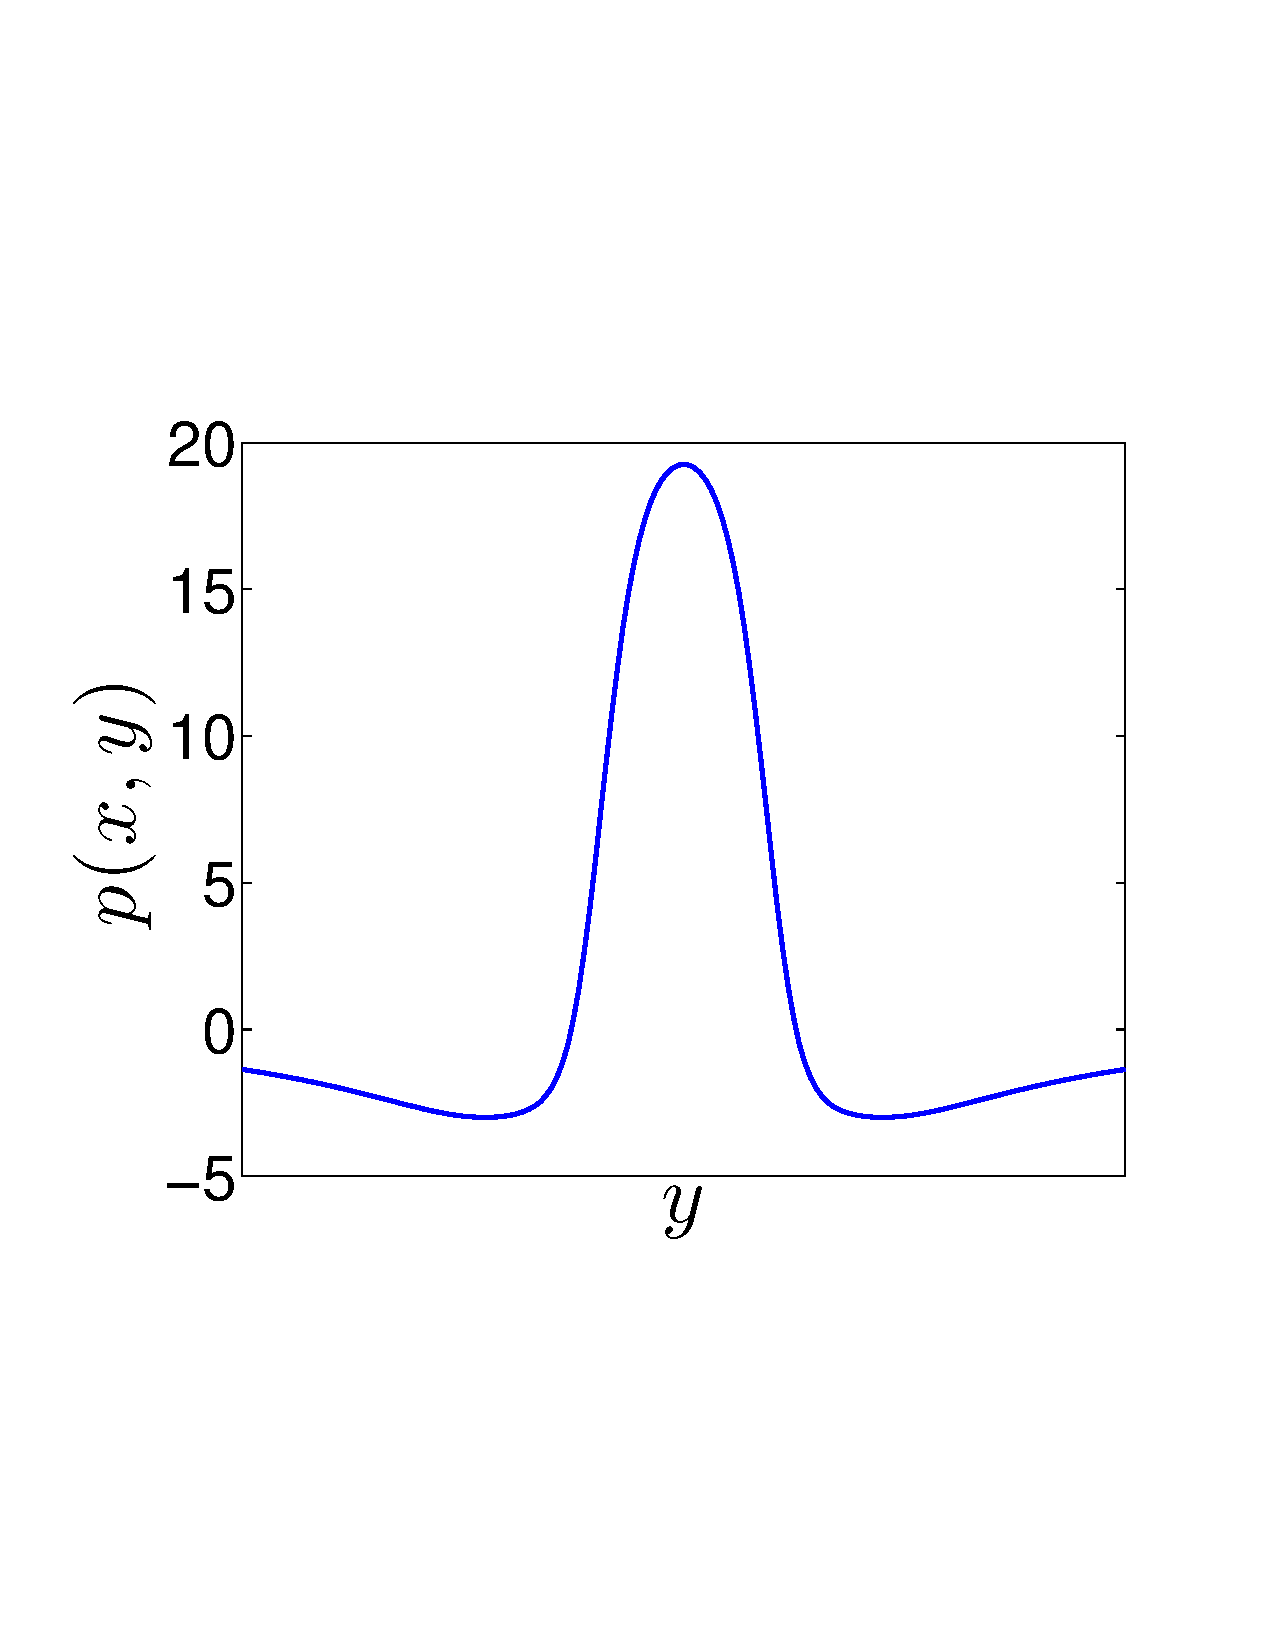
\includegraphics[trim=1.2cm 7cm 2cm 6cm,clip=true,scale = 0.15]{figs/pressurePlotFrame08.pdf} &
  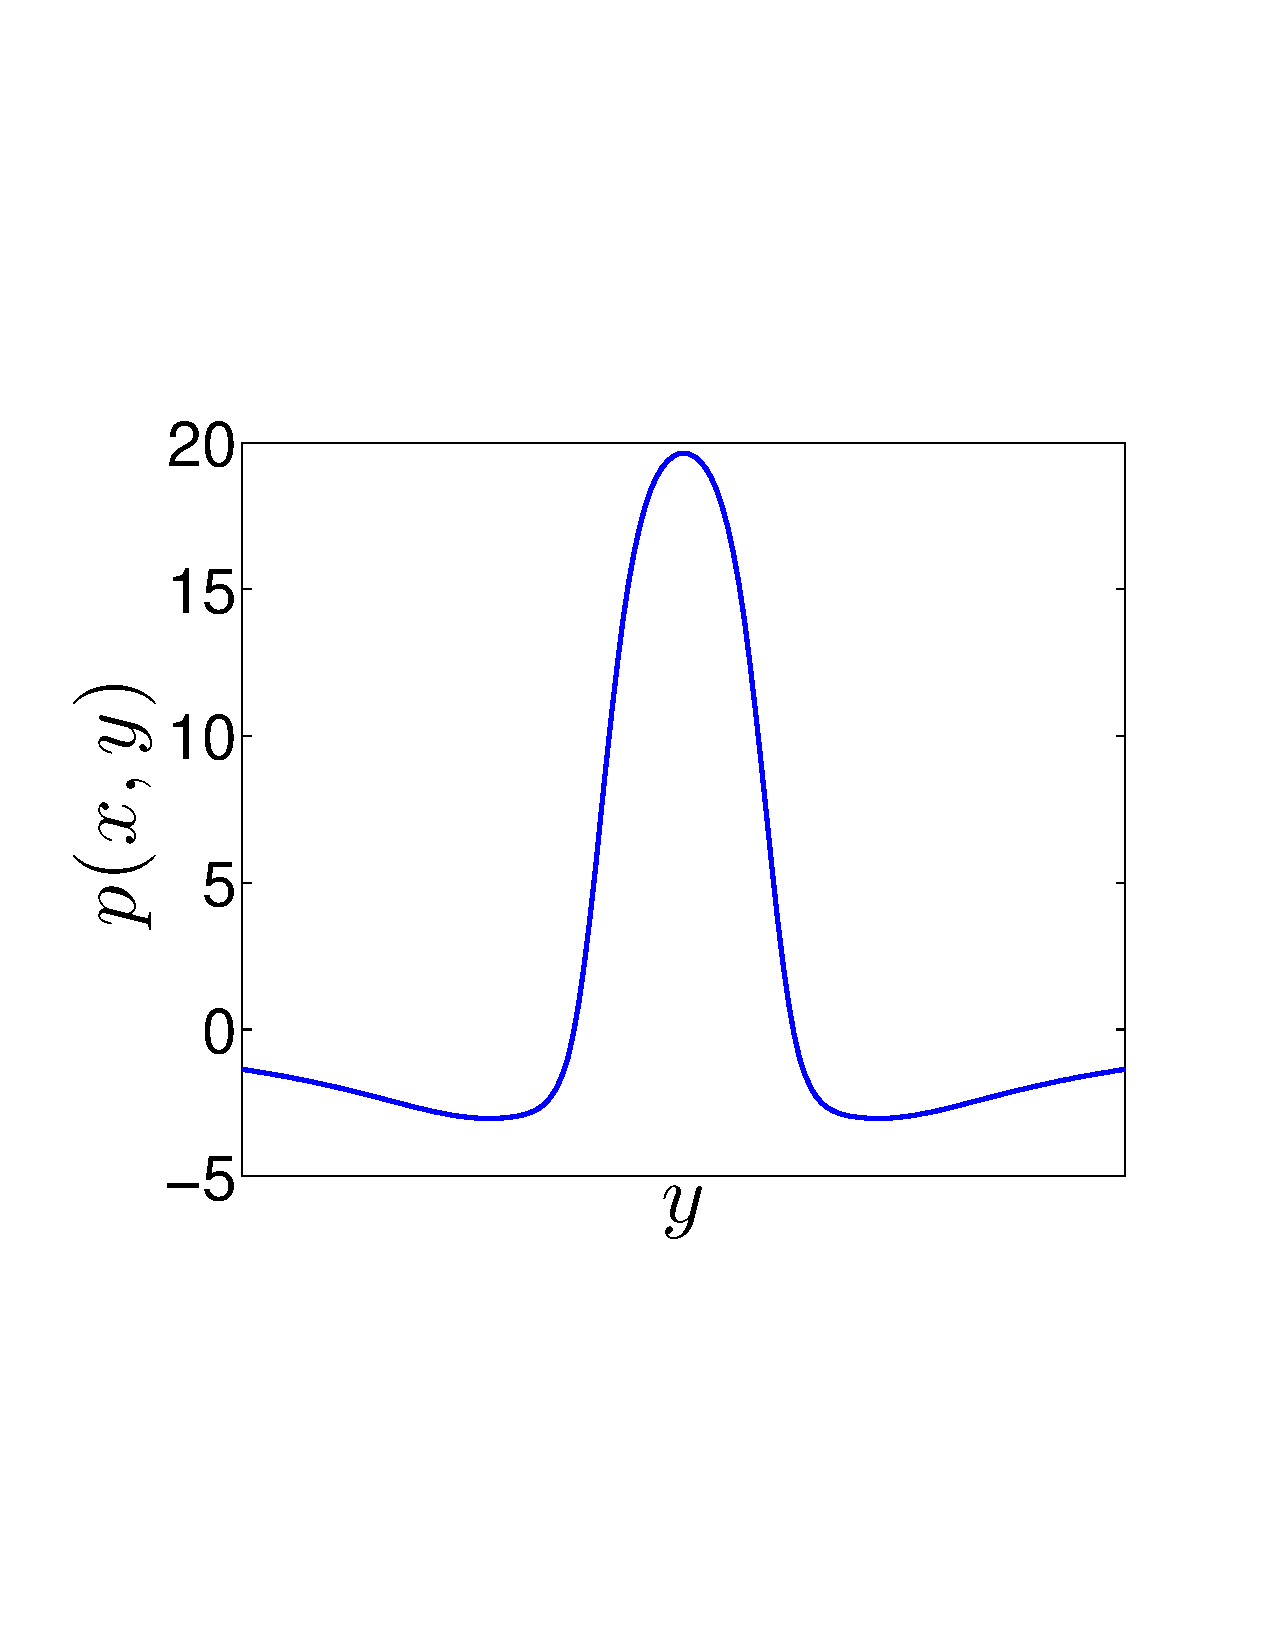
\includegraphics[trim=1.2cm 7cm 2cm 6cm,clip=true,scale = 0.15]{figs/pressurePlotFrame09.pdf} &
  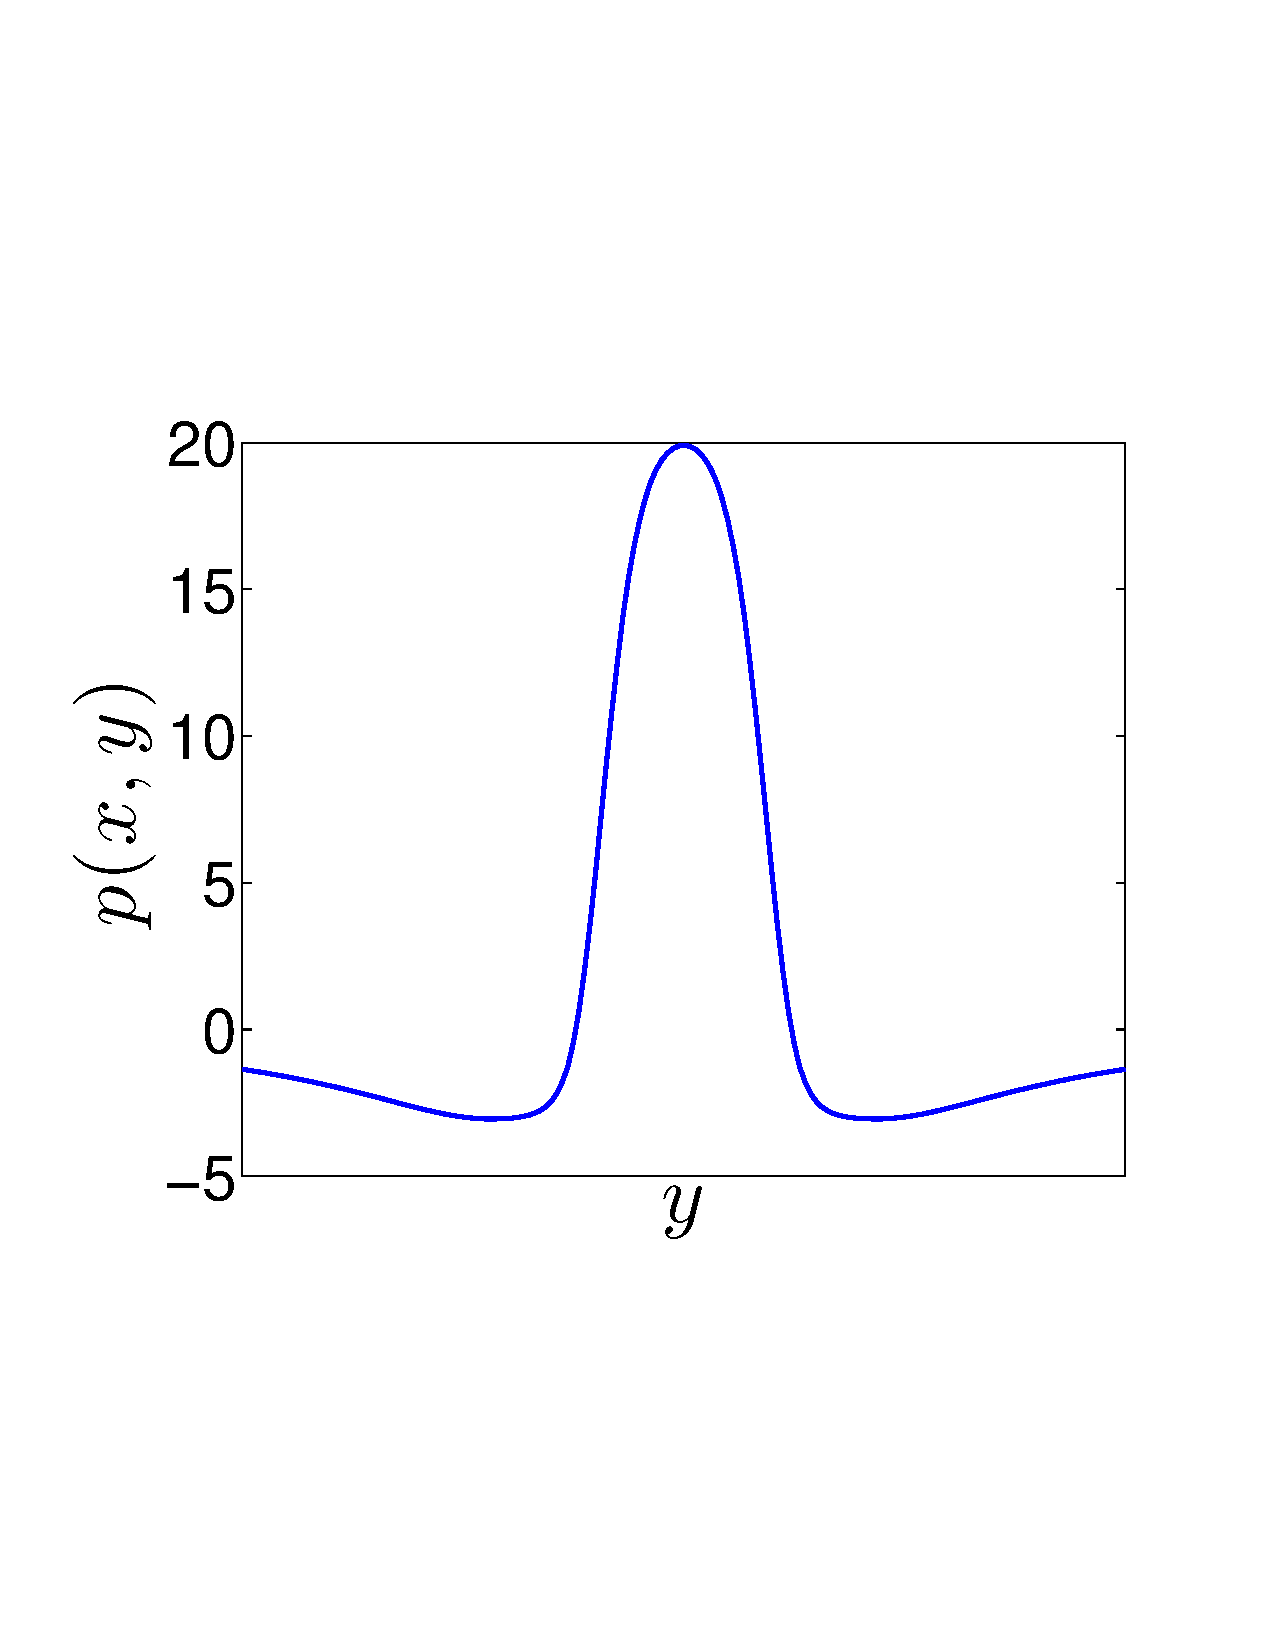
\includegraphics[trim=1.2cm 7cm 2cm 6cm,clip=true,scale = 0.15]{figs/pressurePlotFrame10.pdf} \\ 
\end{array}
$
\mcaption{Contour plots show the pressure in and around the vesicles in
an extensional flow with no viscosity contrast.  The lower plots are
the pressure along the vertical line that passes vertically through the
midpoint of the two vesicles.  We see that the maximum pressure
increases as a function of time and that the pressure inside each
vesicle approaches a constant value.}{f:pressure:figure}
\end{figure}

We now compute the limiting values of the stress tensors
$T^{S}[\ssigma]$ and $T^{D}[\ssigma]$.  The limiting values of
$T^{S}_{q}[\ssigma]$ are
\begin{align}
  \lim_{\substack{\xx \rightarrow \xx_{0} \\ \xx \in \omega_{q}}} 
    T^{S}_{q}[\ssigma](\xx) 
  &=-\frac{1}{2}(\nn_{0} \otimes \ff_{0})\ssigma_{0} +
    \frac{1}{2}\left( \ttau \otimes \left[
    \begin{array}{cc}
      2\tau_{x}\tau_{y} & \tau_{y}^{2} - \tau_{x}^{2} \\
      \tau_{y}^{2} - \tau_{x}^{2} & -2\tau_{x}\tau_{y}
    \end{array}
    \right]\ff_{0} \right) \ssigma_{0} + T^{S}_{q}[\ssigma](\xx_{0}), 
    \label{e:stress:jump:int} \\
  \lim_{\substack{\xx \rightarrow \xx_{0} \\ \xx \notin \omega_{q}}} 
    T^{S}_{q}[\ssigma](\xx) 
  &=\frac{1}{2}(\nn_{0} \otimes \ff_{0})\ssigma_{0} -
    \frac{1}{2}\left( \ttau \otimes \left[
    \begin{array}{cc}
      2\tau_{x}\tau_{y} & \tau_{y}^{2} - \tau_{x}^{2} \\
      \tau_{y}^{2} - \tau_{x}^{2} & -2\tau_{x}\tau_{y}
    \end{array}
    \right]\ff_{0} \right) \ssigma_{0} + T^{S}_{q}[\ssigma](\xx_{0}).
    \label{e:stress:jump:ext}
\end{align}
The jumps are proved in Appendix~\ref{A:AppendixB}.  Since the
singularity at $\xx-\xx_{0}$ is of the order $(\xx - \xx_{0})^{-1}$, we
use odd-even integration to compute the stress on $\gamma_{q}$.  The
jumps in the tensor of the double-layer potential are
\begin{align*}
  \lim_{\substack{\xx \rightarrow \xx_{0} \\ \xx \in \omega_{q}}} 
    T^{D}_{q}[\ssigma](\xx) &= -\frac{\p \ff_{0}}{\p \ttau} \cdot \ttau
    \left(I + \left[
    \begin{array}{cc}
      \tau_{x}^{2}-\tau_{y}^{2} & 2\tau_{x}\tau_{y} \\
      2\tau_{x}\tau_{y} & -\tau_{x}^{2} + \tau_{y}^{2}
    \end{array}
    \right] \right) \ssigma_{0} + T^{D}_{q}[\ssigma](\xx_{0}),
  \\
  \lim_{\substack{\xx \rightarrow \xx_{0} \\ \xx \notin \omega_{q}}} 
    T^{D}_{q}[\ssigma](\xx) &= \frac{\p \ff_{0}}{\p \ttau} \cdot \ttau
    \left(I + \left[
    \begin{array}{cc}
      \tau_{x}^{2}-\tau_{y}^{2} & 2\tau_{x}\tau_{y} \\
      2\tau_{x}\tau_{y} & -\tau_{x}^{2} + \tau_{y}^{2}
    \end{array}
    \right] \right) \ssigma_{0} + T^{D}_{q}[\ssigma](\xx_{0}).
\end{align*}
These jumps are calculated using the jumps $\llbracket p^{D}
\rrbracket$, $\llbracket \uu^{D} \rrbracket$, $\llbracket T^{D}\nn
\rrbracket$, and $\llbracket \grad \cdot \uu^{D} \rrbracket$.  We have
already computed $\llbracket p^{D} \rrbracket$, and the other three
jumps can be found in Appendix B of~\cite{ying-biros-zorin06}.
However, we have to use the same technique we used to compute
$p^{D}(\xx_{0})$ to reduce the order of the singularity of the integral
from $(\xx-\xx_{0})^{-2}$ to $(\xx-\xx_{0})^{-1}$.  Since a constant
hydrodynamic density $\ff$ corresponds to a vanishing stress tensor
$T^{D}$, this modification guarantees that odd-even integration will
converge to the correct value.

We check the convergence rate for the three components of the stress
tensors (the $(1,2)$ and $(2,1)$ entries are identical).  We use the
same vesicle and hydrodynamic density as in
Table~\ref{t:pressure:conv}.  The maximum relative errors are in
Table~\ref{t:stress:conv}.  Since $T^{S},T^{D} \in C^{\infty}$, the
errors in Table~\ref{t:stress:conv} are determined by the order of the
near-singular integration algorithm.  We obtain the expected
$5^{th}$-order convergence.
\begin{table}[htp]
\begin{centering}
\begin{tabular}{lc|cccccc}
& & $N=32$ & $N=64$ & $N=128$ & $N=256$ & $N=512$ & $N=1024$ \\
\hline
Single- & $(1,1)$ & $8.33e-03$ & $6.32e-04$ & $2.40e-05$ & $5.21e-07$ & $4.30e-09$ & $1.23e-14$ \\ 
layer & $(1,2)$ & $5.79e-03$ & $4.24e-04$ & $1.59e-05$ & $3.49e-07$ & $2.89e-09$ & $6.82e-15$ \\ 
potential & $(2,2)$ & $4.39e-03$ & $3.13e-04$ & $1.15e-05$ & $2.49e-07$ & $2.05e-09$ & $1.27e-14$ \\ 
\hline
Double- & $(1,1)$ & $4.22e-03$ & $3.34e-04$ & $1.29e-05$ & $2.81e-07$ & $2.33e-09$ & $1.12e-12$ \\ 
layer & $(1,2)$ & $1.19e-02$ & $8.98e-04$ & $3.42e-05$ & $7.54e-07$ & $6.25e-09$ & $1.75e-12$ \\ 
potential & $(2,2)$ & $9.28e-03$ & $6.80e-04$ & $2.54e-05$ & $5.50e-07$ & $4.54e-09$ & $5.36e-13$ \\ 
\end{tabular}
\mcaption{The maximum relative errors in the calculation of the stress
tensor using near-singular integration along the line $x=1.01$.  The
exact stress is computed analytically using the Residue Theorem.  The
convergence rates are all about $5.2$.  For $N=1024$, the near zone
$\Omega_{0}$ is empty.  This explains the sharp drop in the
errors.}{t:stress:conv}
\end{centering}
\end{table}




